% Created 2021-07-06 Tue 10:54
% Intended LaTeX compiler: pdflatex
\documentclass[11pt]{article}
\usepackage[utf8]{inputenc}
\usepackage[T1]{fontenc}
\usepackage{graphicx}
\usepackage{grffile}
\usepackage{longtable}
\usepackage{wrapfig}
\usepackage{rotating}
\usepackage[normalem]{ulem}
\usepackage{amsmath}
\usepackage{textcomp}
\usepackage{amssymb}
\usepackage{capt-of}
\usepackage{hyperref}
\author{Palak Mathur}
\date{\today}
\title{Internet Security}
\hypersetup{
 pdfauthor={Palak Mathur},
 pdftitle={Internet Security},
 pdfkeywords={},
 pdfsubject={},
 pdfcreator={Emacs 27.2 (Org mode 9.4.4)}, 
 pdflang={English}}
\begin{document}

\maketitle
\tableofcontents


\section{Introduction}
\label{sec:org05fc753}
The Internet was not designed or built with security in mind. Security came as an afterthought after adversaries started misusing or abusing Internet services, resources and infrastructure. All the protocols that we have learned so far can be exploited by attackers for malicious purposes. 

Internet security is a very exciting and active research area and obviously very broad. In this lesson, we focus on specific topics which we will explore through the lenses of what we have known so far in the course. 

Specifically, we focus on attacks that misuse the DNS protocol and the DNS infrastructure. We learn about traffic attraction attacks that are based on BGP abuse. We also learn about the most popular techniques to infer network reputation. Finally, we learn about Denial of Service attacks. Given the increasing popularity of Internet Exchange Points, which we learned about at a previous lesson, we focus on the development of recent DDoS defenses techniques that are offered at IXPs.

An attack on a system aims to compromise properties of a secure communication. 

We discuss how a Domain Name System (DNS) which uses Round Robin DNS (RRDNS) and Content Distribution Networks (CDN) methods can become vulnerable to such attacks. In particular, we look into how Fast Flux networks operate which maintains multiple IP addresses for a single domain name and rapidly changes them. To infer network reputation and thereby the probability of a network abuse, we examine evidence of abuse, interconnection patterns and likelihood of breach as possible approaches. We next focus on the highly critical BGP hijacking attacks which can happen via prefixes advertised by BGP, the AS-path announcements and data-plane traffic manipulation. We go through the possible motivations behind these attacks and try to classify them. We look into a few ideas for detection of BGP hijacking and mitigation techniques such as Prefix deaggregation and Mitigation with Multiple Origin AS (MOAS). To better understand the impact of BGP hijacking, we take up a case study on a real world incident known as the “Linktel Incident” and analyze it. Another category of attacks is the Distributed Denial of Service (DDoS) attack which overloads a server and network resources, making it unavailable for other users. We briefly discuss the different types of DDoS attacks and few mitigation strategies such as filtering, scrubbing and FlowSpec at Internet Exchange Points (IXP). BGP blackholing is a popular defense mechanism which is provided by network providers as well as ISPs and IXPs. In blackholing, the traffic to the target destination is dropped and we go in detail about how blackholing is enabled by BGP. Although this is an effective defense mechanism in case of high volume attacks, it has its own limitations.

\section{Readings and Additional Resources}
\label{sec:org73f0174}

\begin{itemize}
\item Kurose-Ross Edition 6th, Section 8.1

\item \href{https://user.informatik.uni-goettingen.de/\~krieck/docs/2008-ndss.pdf}{Measuring and Detecting Fast-Flux Service Networks}

\item \href{https://sites.cs.ucsb.edu/\~chris/research/doc/acsac09\_fire.pdf}{FIRE: Finding Rogue Networks}

\item \href{https://conferences.sigcomm.org/sigcomm/2015/pdf/papers/p625.pdf}{ASwatch: An AS Reputation System to ExposeBulletproof Hosting ASes}

\item \href{https://www.usenix.org/system/files/conference/usenixsecurity15/sec15-paper-liu.pdf}{Cloudy with a Chance of Breach: Forecasting Cyber Security Incident}

\item \href{https://www.inspire.edu.gr/wp-content/pdfs/artemis\_TON2018.pdf}{ARTEMIS: Neutralizing BGP HijackingWithin a Minute}

\item \href{https://www.researchgate.net/profile/Bahaa\_Musawi/publication/309519246\_BGP\_Anomaly\_Detection\_Techniques\_A\_Survey/links/5a63db73aca272a1581bf3ea/BGP-Anomaly-Detection-Techniques-A-Survey.pdf}{BGP Anomaly Detection Techniques: A Survey}

\item \href{http://www.sigcomm.org/sites/default/files/ccr/papers/2013/April/2479957-2479959.pdf}{A Forensic Case Study on AS Hijacking:The Attacker’s Perspective}

\item \href{https://www.icir.org/vern/papers/reflectors.CCR.01.pdf}{An Analysis of Using Reflectors for Distributed Denial-of-Service Attacks}

\item \href{https://www.de-cix.net/Files/2731074c857497be3827ac9537b6e486f27aa57c/Research-paper-Stellar-Network-Attack-Mitigation-using-Advanced-Blackholing.pdf}{Stellar: Network Attack Mitigation using Advanced Blackholing}

\item \href{https://www.de-cix.net/Files/3dc6302479dc77225a799f83532945dbcb6ea236/Inferring-BGP-Blackholing-Activity.pdf}{Inferring BGP Blackholing Activity in the Internet}

\item \href{https://ripe78.ripe.net/presentations/9-RIPE\_Presentation\_MW.pdf}{Next Gen Blackholing to Counter DDoS}
\end{itemize}

\section{Properties of Secure Communication}
\label{sec:org8c90464}

When establishing a communication, there are certain properties that are important to ensure so the communication is secure even in the presence of attackers:

\begin{enumerate}
\item \textbf{Confidentiality} – This is perhaps the first thing that comes to our mind when we think about a secure communication. We want to ensure that the message that is sent from the sender to the receiver is only available to the two parties. An attack scenario is that we have an intruder that can eavesdrop on the communication by sniffing or recording the exchanged messages. One measure to increase the chances that a communication is confidential is to encrypt the message so that even if the communication is intercepted, the message would be meaningless to the attacker.
\item \textbf{Integrity} – In addition to confidentiality, it is important to ensure the message has not been somehow modified while in transit from the sender to the receiver. For example, an intruder could attack by modification, insertion or deletion of part of the messages send. As a countermeasure, we can introduce mechanisms that check for the integrity of the message.
\item \textbf{Authentication} – When two parties are communicating, it is important to ensure that the two parties are who they say they are. For example, an intruder may try to steal information by impersonating another entity on the network. As a countermeasure against these attacks we use authentication mechanisms to verify the identity of a user.
\item \textbf{Availability} - A communication is not useful unless the information (or the service that is provided) is indeed available. So we will need to ensure that multiple aspects of the communication channel are functioning appropriately and we can cope with possible failures such as power outages, hardware failures, etc. or attacks that aim to render the system unavailable such as denial of service attacks.
\end{enumerate}

In the following sections we will see examples about attackers abuse several of the protocols that we have learned so far for malicious purposes.

Each of these abuses may prohibit one or more of the desired properties of secure communication. 

\begin{figure}[htbp]
\centering
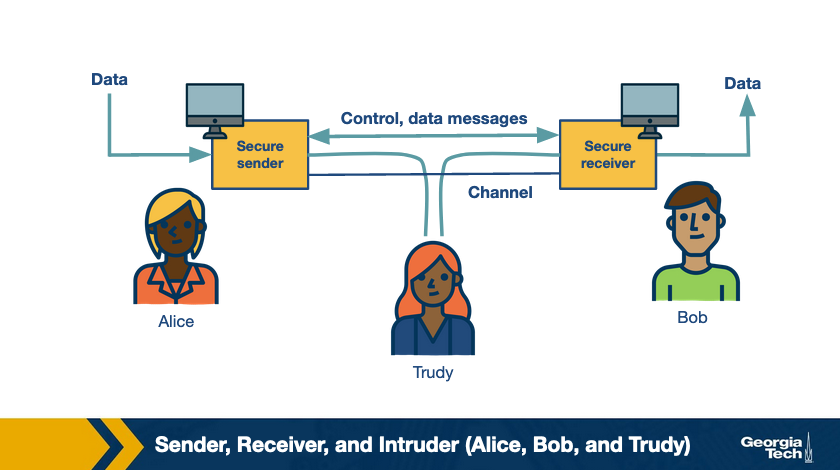
\includegraphics[width=.9\linewidth]{./MD_Figures/9_properties_secure_comm_1.png}
\caption{\label{fig:org399970c}Sender, Receiver, and Intruder (Alice, Bob, and Trudy)}
\end{figure}



\section{DNS Abuse}
\label{sec:org521f7a2}

We will start our discussion with DNS abuse.

Attackers have developed techniques abusing the DNS protocol so to extend the uptime of domains that are used for malicious purposes (e.g. Command and Control hosting infrastructure, phishing, spamming domains, hosting illegal businesses, illegal content). The ultimate goal of this abuse is to remain undetectable for longer.

In this lecture we will talk about some of the techniques that the attackers have developed to abuse DNS. These techniques have their roots in legitimate DNS-based techniques that legitimate businesses and administrators use. We will start by talking about legitimate techniques before seeing how attackers are twisting them for their own malicious purposes.

\section{Round Robin DNS (RRDNS)}
\label{sec:orgb6ea00b}

This method is used by large websites to distribute the load of incoming requests to several servers at a single physical location. It responds to a DNS request with a list of DNS A records, which it then cycles through in a round robin manner. The DNS client can then choose a record using different strategies –choose the first record each time, use the closest record in terms of network proximity, etc. Each A record also has a Time to Live (TTL) for this mapping which specifies the number of seconds the response is valid. If the lookup is repeated while the mapping is still active, the DNS client will receive the same set of records, albeit in a different order.

\section{DNS-based content delivery}
\label{sec:org48f1caf}

Content Distribution Networks (CDNs) also use DNS-based techniques to distribute content but using more complex strategies. For example, CDNs distribute the load amongst multiple servers at a single location, but also distribute these servers across the world. When accessing the name of the service using DNS, the CDN computes the ‘nearest edge server’ and returns its IP address to the DNS client. It uses sophisticated techniques based on network topology and current link characteristics to determine the nearest server. This results in the content being moved ‘closer’ to the DNS client which increases responsiveness and availability. CDNs can react quickly to changes in link characteristics as their TTL is lower than that in RRDNS. 

\section{Fast-Flux Service Networks}
\label{sec:orgf71fe4c}

The previous two strategies provide reliability, scalability and resilience, which is great for larger websites. However, this also benefits spammers. Since using these techniques, a DNS request receives multiple A records (each containing a different IP address), this makes it harder to shut down online scams, as if even one IP address is functional, the scam is still working. Similarly, spreading across several servers makes the shutdown of these scams more complex!

Fast-Flux Service Networks (FFSN) is an extension of the ideas behind RRDNS and CDN. As its name suggests, it is based on a ‘rapid’ change in DNS answers, with a TTL lower than that of RRDNS and CDN. One key difference between FFSN and the other methods is that after the TTL expires, it returns a different set of A records from a larger set of compromised machines. These compromised machines act as proxies between the incoming request and control node/mothership, forming a resilient, robust, one-hop overlay network.


\begin{figure}[htbp]
\centering
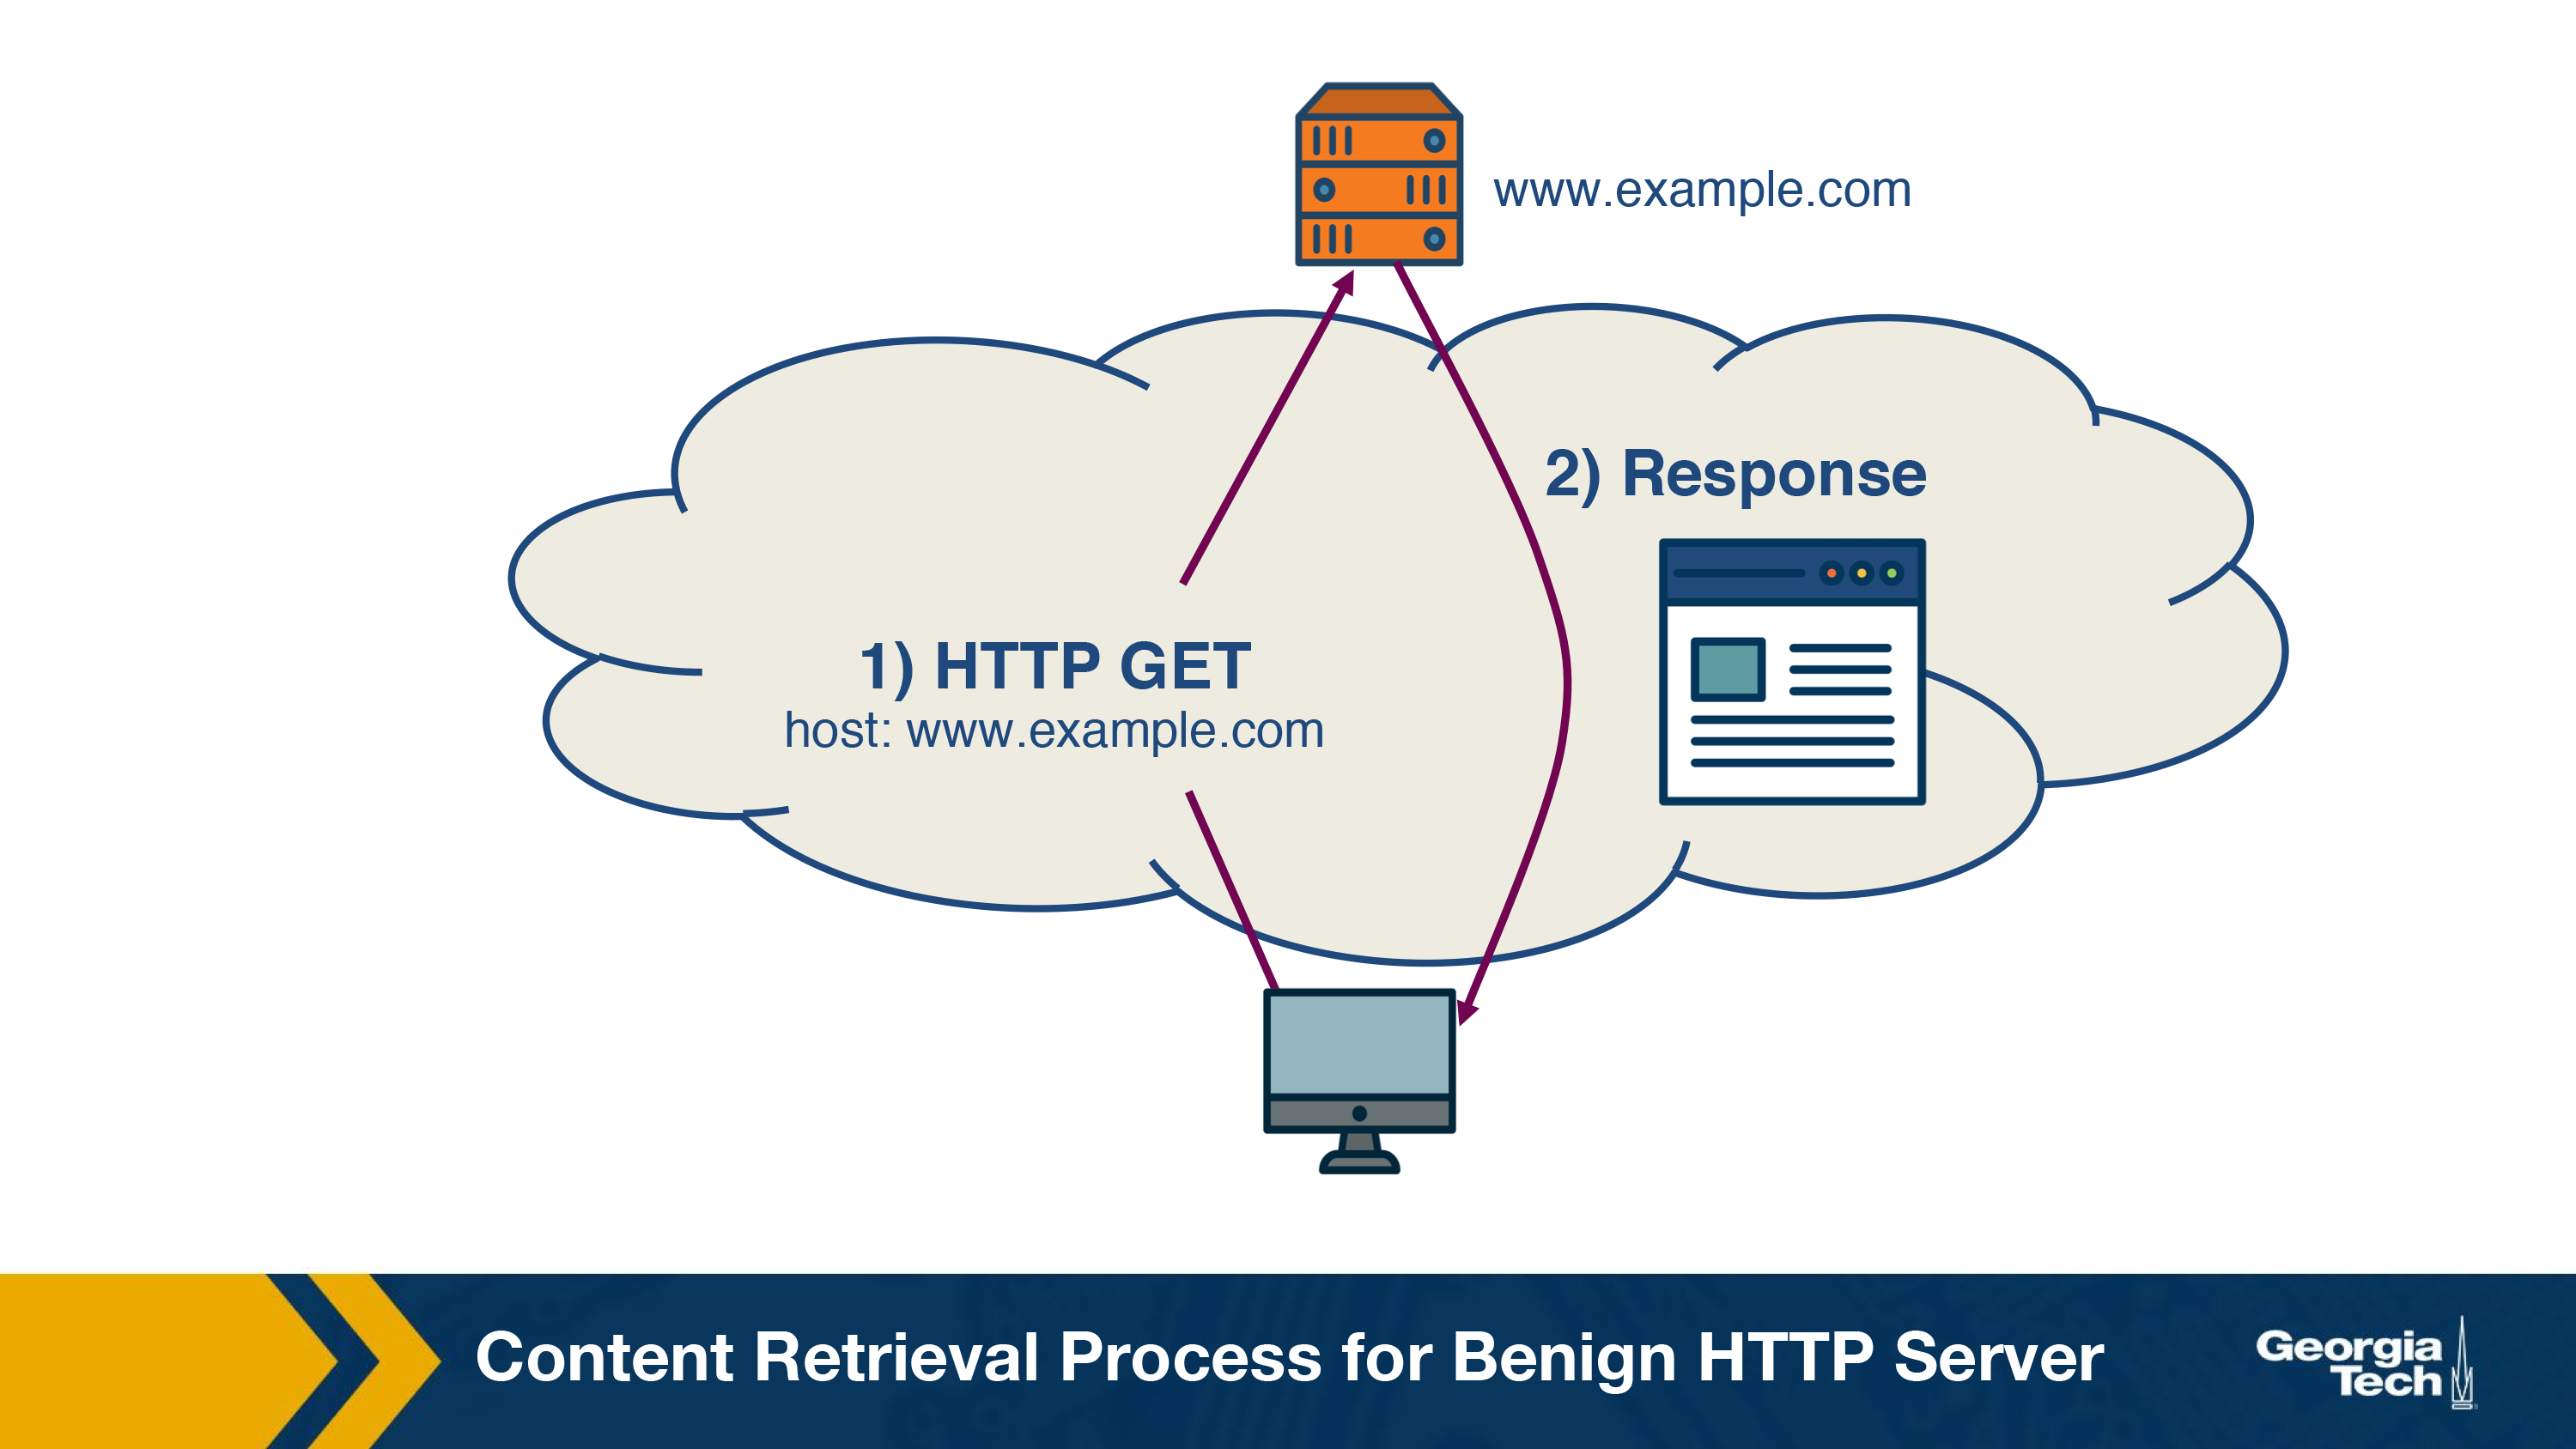
\includegraphics[width=.9\linewidth]{./MD_Figures/9_dns_abuse_1.png}
\caption{\label{fig:orgc301143}The figure above shows the content retrieval process of a benign HTTP server. The DNS lookup returns the IP address of the control node of that domain, and the request – HTTP GET is sent to this control node. The control node responds directly to the incoming request with the content of the domain.}
\end{figure}


\begin{figure}[htbp]
\centering
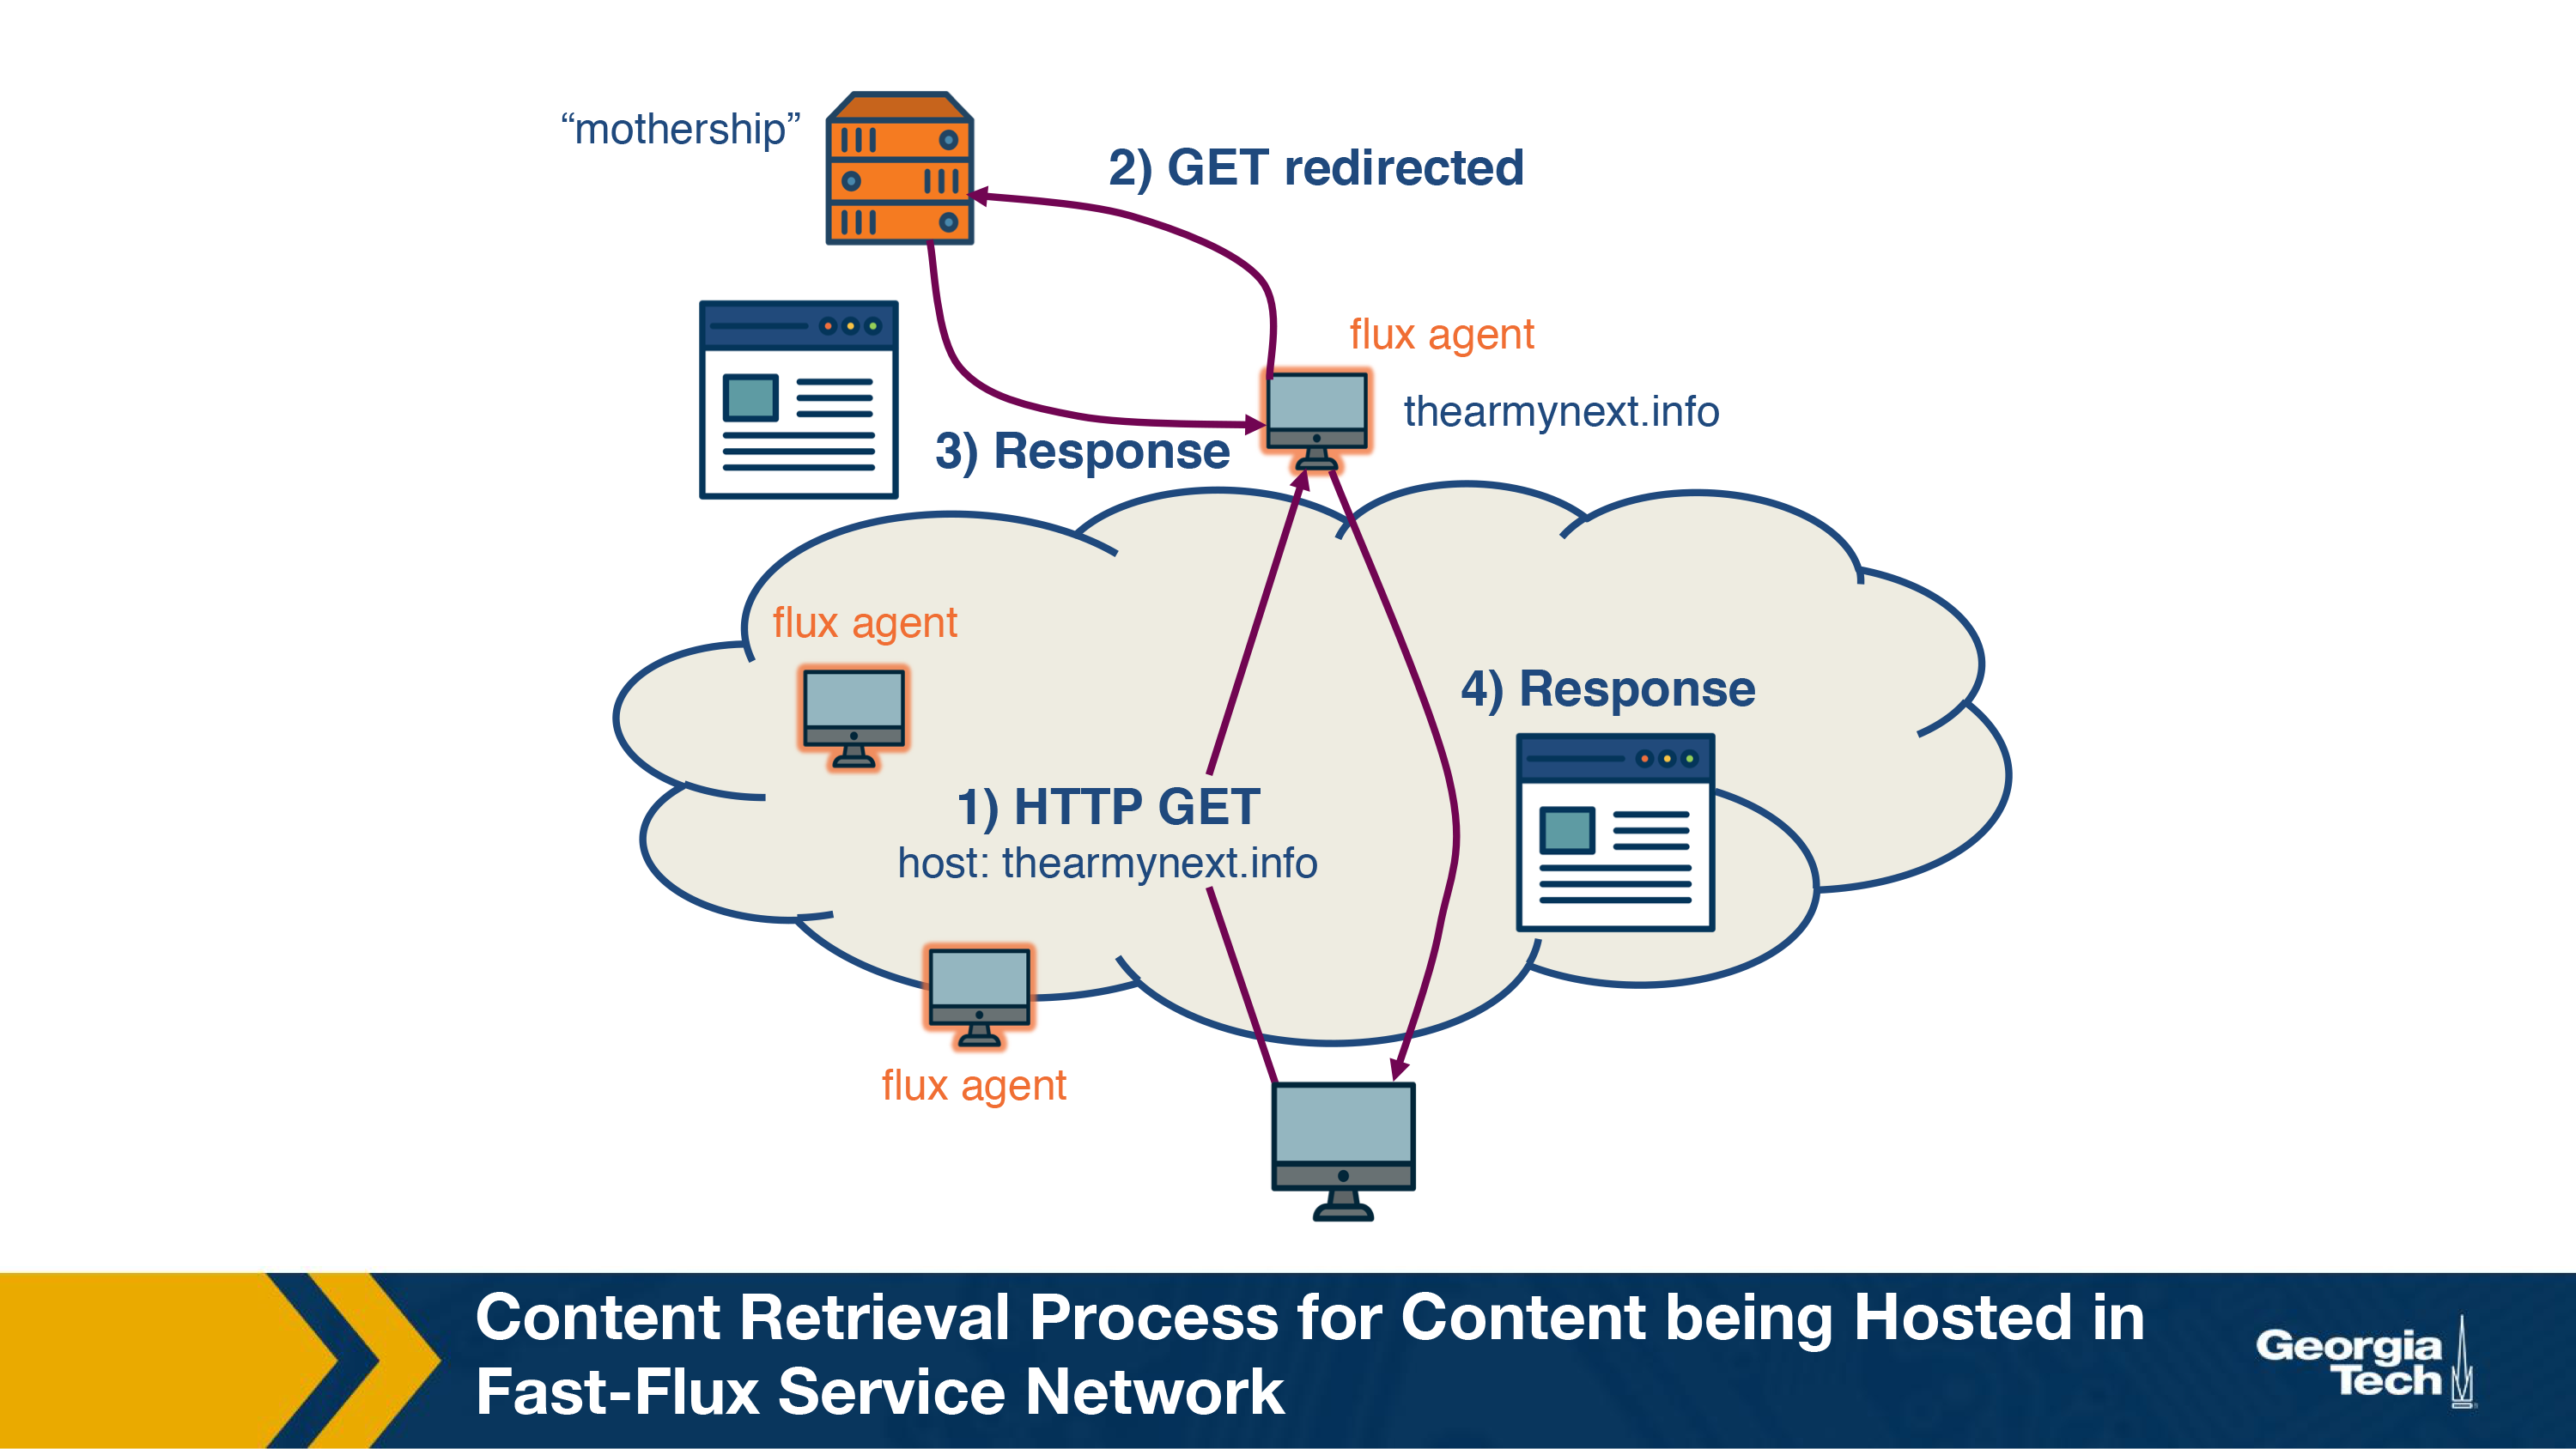
\includegraphics[width=.9\linewidth]{./MD_Figures/9_dns_abuse_2.png}
\caption{\label{fig:org3abc039}The figure above shows the content-retrieval process for content hosted in a FFSN. The domain ‘www.thearmynext.info’ was found in a spam email. Here, the mothership is the control node where the actual content of the scam is being hosted. The DNS lookup from the client returns several different IP addresses, all belonging to compromised machines in the network (flux agents). Each time the TTL expires, the lookup returns completely different IP addresses. The flux-agent then relays the request it receives (HTTP GET) to the control node, which sends content to the flux-agent. Lastly, the content is delivered to the client. It is interesting to note that these flux agents, although seemingly close to each other, are usually located in different countries and belong to different Autonomous Systems (AS).}
\end{figure}

An important aspect of Internet abuse is the infrastructure that attackers use to support the abuse. For example, the attackers need Internet infrastructure to support illegal content hosting, C\&C infrastructure hosting, etc. 

Next we will talk about approaches that have been suggested to infer network reputation, and hence the likelihood that a network will be abused to facilitate attacks.


\section{How to Infer Network Reputation: Evidence of Abuse}
\label{sec:orgb9eafce}

In this section, we discuss FIRE – FInding Rogue nEtworks, a system that monitors the Internet for rogue networks. Rogue networks are networks whose main purpose is malicious activity such as phishing, hosting spam pages, hosting pirated software, etc. It uses three main data sources to identify hosts that likely belong to rogue networks:

\begin{enumerate}
\item \textbf{Botnet command and control providers}
\end{enumerate}

Several botnets still rely on centralized command and control (C\&C). So a bot-master would prefer to host their C\&C on networks where it is unlikely to be taken down. The two main types of botnets this system considers are IRC-based botnets and HTTP-based botnets.

\begin{enumerate}
\item \textbf{Drive-by-download hosting providers}
\end{enumerate}

Drive-by-download is a method of malware installation without interaction with the user. It commonly occurs when the victim visits a web page that contains an exploit for their vulnerable browser. 

\begin{enumerate}
\item \textbf{Phish housing providers}
\end{enumerate}

This data source contains URLs of servers that host phishing pages. Phishing pages usually mimic authentic sites to steal login credentials, credit card numbers and other personal information. These pages are hosted on compromised servers and usually are up only for a short period of time. 

The key difference between rogue and legitimate networks is the longevity of malicious behavior. Legitimate networks are usually able to remove the malicious content within a few days whereas rogue networks may let the content be up for weeks to more than a year! By disregarding IP addresses that have been active for a short time, we ignore phishing attacks hosted on legitimate networks and web servers that were temporarily abused for botnet communication. 

Each of these data sources produces a list (Li) of malicious IP addresses daily. FIRE combines the information from these three lists to identify rogue AS (organizations are considered equivalent to autonomous systems). The approach is to identify the most malicious networks as those which have the highest ratio of malicious IP addresses as compared to the total owned IP addresses of that AS. 

\section{How to Infer Network Reputation: Interconnection Patterns}
\label{sec:org763967c}

In this topic, we continue our discussion on approaches to infer network reputation. In an earlier topic, we discussed an approach that is based on data plane monitoring. With data plane monitoring only if a network has a large enough concentration of blacklisted IPs it will be flagged as malicious. We flag a network as malicious only after we have observed indications of malicious behavior for a long enough period of time. For example, let's say we have access to a blacklist and we observe a large number of IPs that belong to an AS to be blacklisted for spamming, phishing, hijacking, etc. 

But in practice, it is not feasible to monitor the traffic of all networks to detect malicious behaviors from the data plane. In addition, the disadvantage of this approach is that it may take a long time until a very large fraction of IPs makes it to a blacklist, and 2) the approach does not differentiate well between networks that are legitimate but abused, and those which are likely operated by cyberactors. 

This topic discusses a complementary approach – ASwatch which uses information exclusively from the control plane (ie. routing behavior) to identify malicious networks. Also, this approach aims to detect malicious networks that are likely run by cyberactors, or \texttt{bulletproof} as they are called, rather than networks that may be badly abused.

\begin{figure}[htbp]
\centering
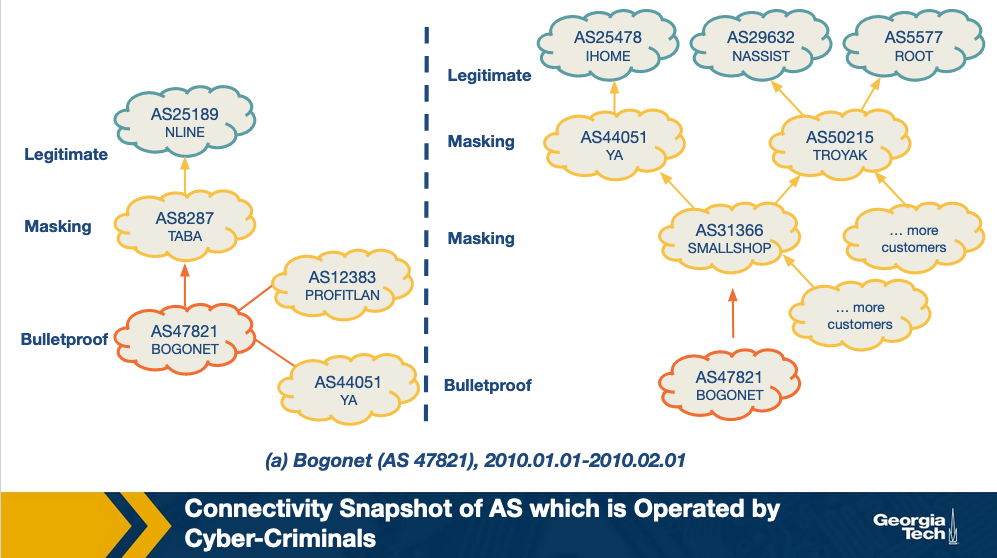
\includegraphics[width=.9\linewidth]{./MD_Figures/9_interconnection_patterns_1.png}
\caption{\label{fig:orgbdf959a}Connectivity Snapshot of AS which is operated by Cyber Criminals}
\end{figure}
\begin{figure}[htbp]
\centering
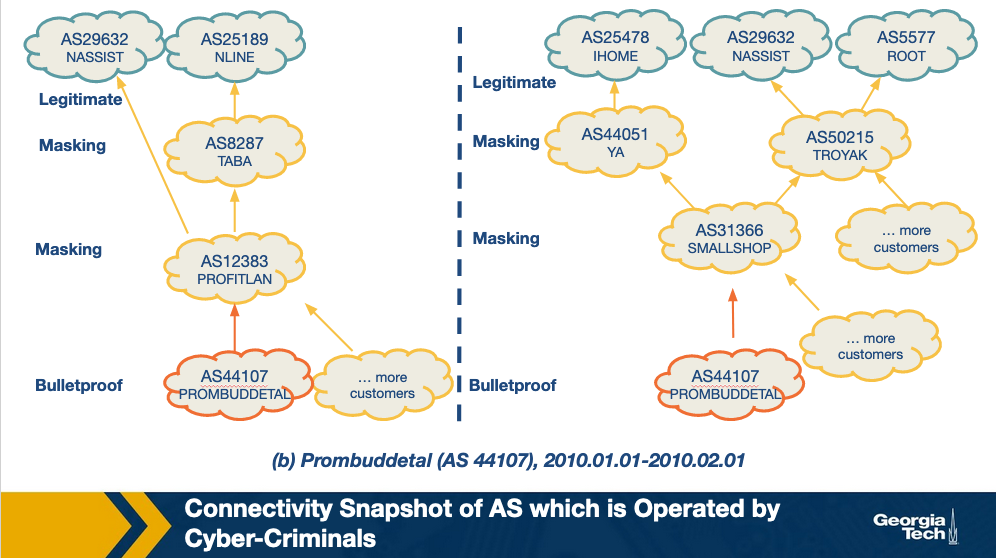
\includegraphics[width=.9\linewidth]{./MD_Figures/9_interconnection_patterns_2.png}
\caption{\label{fig:orgbdf959a}Connectivity Snapshot of AS which is operated by Cyber Criminals}
\end{figure}
\begin{figure}[htbp]
\centering
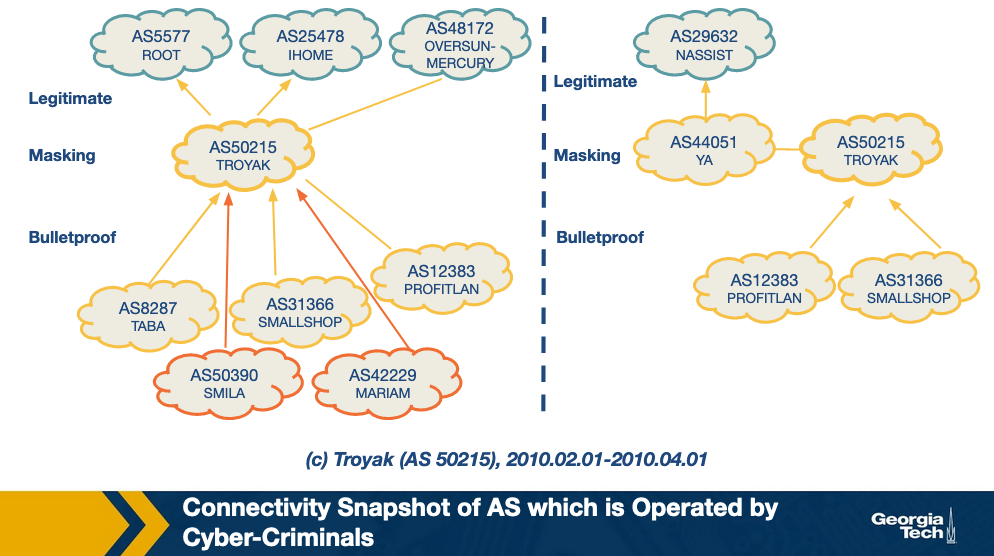
\includegraphics[width=.9\linewidth]{./MD_Figures/9_interconnection_patterns_3.png}
\caption{\label{fig:orgbdf959a}Connectivity Snapshot of AS which is operated by Cyber Criminals}
\end{figure}

The approach is based on the observation that bulletproof ASes have distinct interconnection patterns and overall different control plane behavior from most legitimate networks. For example, let's observe example snapshots of the topology around known bulletproof networks, that are taken a few months apart. These networks shown as red in the figures are found to be changing upstream providers more aggressively than most legitimate networks, also they are found to behave customer-provider or peering relationships with likely shady networks, rather than connecting with directly with legitimate networks. These behaviors help the bulletproof network to remain unnoticeable for longer, and when complaints may start, the bulletproof network can simply change an upstream provider.

The design of ASwatch is based on monitoring global BGP routing activity to learn the control plane behavior of a network. The system has two phases:

\begin{enumerate}
\item \textbf{Training phase} - The system learns control-plane behavior typical of both types of ASes. The system is given a list of known malicious and legitimate ASes. It then tracks the behavior of these ASes over time to track their business relationships with other ASes and their BGP updates/withdrawals patterns.  ASwatch then computes statistical features of each AS. There are three main families of features:
\end{enumerate}

a. \textbf{Rewiring activity} – based on changes in the AS connecting activity. Frequent changes in customers/providers, connecting with less popular providers, etc. is usually suspicious behavior.

b. \textbf{IP Space Fragmentation and Churn} - based on the advertised prefixes. Malicious ASes are likely to use small BGP prefixes to partition their IP address space and only advertise a small section of these (to avoid all of them being taken down at one if detected).

c. \textbf{BGP Routing Dynamics} – The BGP announcements and withdrawals for malicious ASes follow different patterns from legitimate ones – such as periodically announcing prefixes for short periods of time.

The system then uses supervised learning to capture the known behaviors and patterns with a trained model.   

\begin{enumerate}
\item \textbf{Operational phase} - Given an unknown AS, it then calculates the features for this AS. It uses the model to then assign a reputation score to the AS. If the system assigns the AS a low reputation score for several days in a row (indicating consistent suspicious behavior), it identifies it as malicious.
\end{enumerate}

\section{How to Infer Network Reputation: Likelihood of Breach}
\label{sec:orgbd70231}

In this section, we look at a system to predict the likelihood of a security breach within an organization (such as the JP Morgan Chase attack that affected almost 76 million households), by using only externally observable features. This is important, as it allows the model to be scalable to all organizations! The system uses these features to train a Random Forest and predict the likelihood.

There are 3 classes of features used for this model:

\begin{enumerate}
\item \textbf{Mismanagement symptoms} – If there are misconfigurations in an organization’s network, it indicates that there may not be policies in place to prevent such attacks or may not have the technological capability to detect these failures. This increases the likelihood of a breach. The features used are:

i. \textbf{Open Recursive Resolvers} – misconfigured open DNS resolvers

ii. \textbf{DNS Source Port Randomization} – many servers still do not implement this

iii. \textbf{BGP Misconfiguration} – short-lived routes can cause unnecessary updates to the global routing table.

iv. \textbf{Untrusted HTTPS Certificates} – can detect the validity of a certificate by TLS handshake.

v. \textbf{Open SMTP Mail Relays} – servers should filter messages so that only those in the same domain can send mails/messages.

\item \textbf{Malicious Activities} – Another factor to consider is the level of malicious activities that are seen to originate from the organization’s network and infrastructure. We can determine this using spam traps, darknet monitors, DNS monitors, etc. We create a reputation blacklist of the IP addresses that are involved in some malicious activities. There are 3 such types of malicious activities:

i. Capturing spam activity – for example, CBL, SBL, SpamCop

ii. Capturing phishing and malware activities – for example, PhishTank, SURBL

iii. Capturing scanning activity – for example, Dshield, OpenBL

\item \textbf{Security Incident Reports} – Data based on actual security incidents gives us the ground truth on which to train our machine learning model on. The system uses 3 collections of such reports to ensure a wider coverage area:

i. \textbf{VERIS Community Database} – This is a public effort to collect cyber security incidents in a common format. It is maintained by the Verizon RISK team. It contains more than 5000 incident reports.

ii. \textbf{Hackmageddon} – This is an independently maintained blog that aggregates security incidents on a monthly basis.

iii. \textbf{The Web Hacking Incidents Database} – This is an actively maintained repository for cyber security incidents.
\end{enumerate}

This system uses a Random Forest (RF) classifier and compares it to a baseline provided by a Support Vector Machine (SVM). It uses 258 features – the features described above (divided into features based on the timespan for which they are valid), secondary features based on statistics from the other features, and the size of the organization. These inputs are processed, then fed to a RF which produces a risk probability (a float). By thresholding this value, we obtain the binary class label. Since this data is sequential, the training-testing splits of the data are strictly based on the time of each datapoint. The best combination of parameters gives this model an accuracy of 90\%!

\section{Traffic Attraction Attacks: BGP Hijacking}
\label{sec:orgf272998}

BGP hijacking attacks can be classified into the following groups:

\begin{enumerate}
\item \textbf{Classification by Affected Prefix}: In this class of hijacking attacks, we are primarily concerned with the IP prefixes that are advertised by BGP. There are different ways the prefix can be targeted, such as:
\end{enumerate}

a. \textbf{Exact prefix hijacking}: When two different ASes (one is genuine and the other one is counterfeit) announce a path for the same prefix. This disrupts routing in such a way that traffic is routed towards the hijacker wherever the AS-path route is shortest, thereby disrupting traffic.

b. \textbf{Sub-prefix hijacking}: This is an extension of exact prefix hijacking, except that in this case, the hijacking AS works with a sub-prefix of the genuine prefix of the real AS. This exploits the characteristic of BGP to favor more specific prefixes, and as a result route large/entire amount of traffic to the hijacking AS.

Example: A given hijacking AS labelled AS2 announces that it has a path to prefix 10.10.0.0/24 which is a part of 10.10.0.0/16 owned by AS1.

c. \textbf{Squatting}: In this type of attack, the hijacking AS announces a prefix that has not yet been announced by the owner AS.

\begin{enumerate}
\item \textbf{Classification by AS-Path announcement}: In this class of attacks, an illegitimate AS announces the AS-path for a prefix for which it doesn’t have ownership rights. There are different ways this can be achieved:
\end{enumerate}

a. \textbf{Type-0 hijacking}: This is simply an AS announcing a prefix not owned by itself.

b. \textbf{Type-N hijacking}: This is an attack where the counterfeit AS announces an illegitimate path for a prefix that it does not own to create a fake link (path) between different ASes.

For example, \{AS2, ASx, ASy, AS1 – 10.0.0.0/23\} denotes a fake path between AS2 and AS1, where there is no link between AS2 and ASx. The N denotes the position of the rightmost fake link in the illegitimate announcement, e.g. \{AS2, ASy, AS1 – 10.0.0.0/23\} is a Type-2 hijacking.

c. \textbf{Type-U hijacking}: In this attack the hijacking AS does not modify the AS-PATH but may change the prefix.



\begin{enumerate}
\item \textbf{Classification by Data-Plane traffic manipulation}: In this class of attacks, the intention of the attacker is to hijack the network traffic and  manipulate the redirected network traffic on its way to the receiving AS. There are three ways the attack can be realized under this classification, i.e.   traffic intercepted by the hijacker can be
\end{enumerate}

a. \textbf{Dropped}, so that it never reaches the intended destination. This attack falls under the category of blackholing (BH) attack.

b. \textbf{Eavesdropped or manipulated} before it reaches the receiving AS, which is also called as man-in-the-middle attack (MM).

c. \textbf{Impersonated}, e.g. In this case the network traffic of the victim AS is impersonated and the response to this network traffic is sent back to the sender. This attack is called imposture (IM) attack.

\section{Traffic Attraction Attacks: Motivations}
\label{sec:org8eaf1e2}

In the previous section, we looked at the types of BGP hijacking attacks, and how to characterize them individually. In this section, we are interested in understanding the \textbf{causes or motivations behind these attacks}. Broadly viewed, the attacks can be classified as caused by:

\begin{enumerate}
\item \textbf{Human Error}: This is an accidental routing misconfiguration due to manual errors. This can lead to large scale exact-prefix hijacking. e.g: China Telecom accidentally leaked a full BGP table that led to large-scale Type-0 hijacking
\item \textbf{Targeted Attack}: In this type of attack, the hijacking AS usually intercepts network traffic (MM attack) while operating in stealth mode to remain under the radar on the control plane (Type-N and Type-U attacks). e.g: Visa and Mastercard’s traffic were hijacked by Russian networks using this method in 2017
\item \textbf{High Impact Attack}: Here, the attacker is obvious in their intent to cause widespread disruption of services. e.g: Pakistan Telecom in a Type-0 sub-prefix hijacking, essentially blackholing all of YouTube’s services worldwide for nearly 2 hours.
\end{enumerate}

To summarize, we can say that the motivation behind every hijacking attempt is different, so there is no one answer when it comes to choosing the best attack. Given the constraining scenario and intents of the hijacking attempt, the hijacker may employ one or a combination of methods to carry out the attack.

\section{Example BGP Hijack Attacks}
\label{sec:org247c69b}

We briefly looked at the different types of BGP hijacking attacks in the previous section. Let's look at how these attacks are carried out through some examples. 

Let's first look at a legitimate scenario. In the figure below, we have a new prefix being announced by an AS to its neighbors:

\begin{enumerate}
\item AS1 announces a new prefix (10.10.0.0/16)
\item AS2, AS3, AS4 and AS5 that receive an announcement from the previous / neighboring AS, check whether this entry is present in the RIB, if new, add it, and send it to all neighboring ASes.
\item As the announcements are made by AS2, AS3 and AS4; A5 eventually receives the full path and new prefix from A4 (4,2,1).
\item If multiple routes exist for a prefix, then the selected (best) route is highlighted. Also, this route is selected for announcement to the neighbors.

\begin{figure}[htbp]
\centering
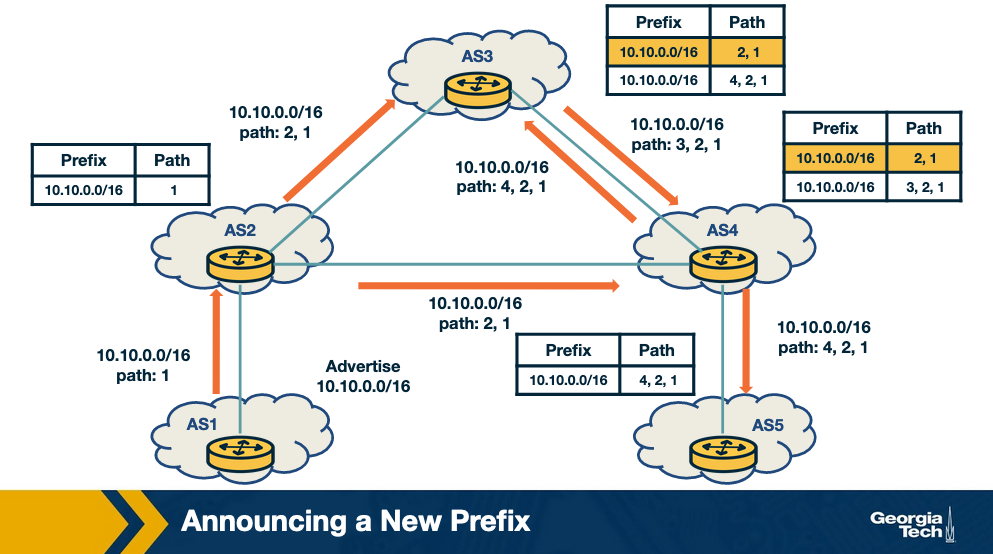
\includegraphics[width=.9\linewidth]{./MD_Figures/9_bgp_attacks_1.png}
\caption{\label{fig:org3878b32}Announcing a new prefix}
\end{figure}
\end{enumerate}

\subsection{Attack Scenario: Hijacking a prefix}
\label{sec:orgafae2b5}

Let's look at the scenario of prefix hijacking. In this scenario, the attacker uses a router at AS4 to send false announcements and hijack the prefix 10.10.0.0/16 that belongs to AS1.  

\begin{enumerate}
\item The attacker uses a router to announce the prefix 10.10.0.0/16 that belongs to AS1, with a new origin AS4, pretending that the prefix belongs to AS4.
\item This new announcement causes a conflict of origin for the ASes that receive it (Multiple Origin AS or MOAS).
\item As a result of the new announcement, AS2, AS3 and AS5 receive the false advertisement and they compare it with the previous entries in their RIB.
\item AS2 will not select the route as the best route as it has the same path length with an existing entry.
\item AS3 and AS5 will believe the new advertisement, and they will update their entries (10.10.0.0/16 with path 4,2,1) to (10.10.0.0/16 with path 4). Therefore AS5 and AS3 will send all traffic for prefix 10.10.0.0/16 to AS4 instead of AS1.
\end{enumerate}


\begin{figure}[htbp]
\centering
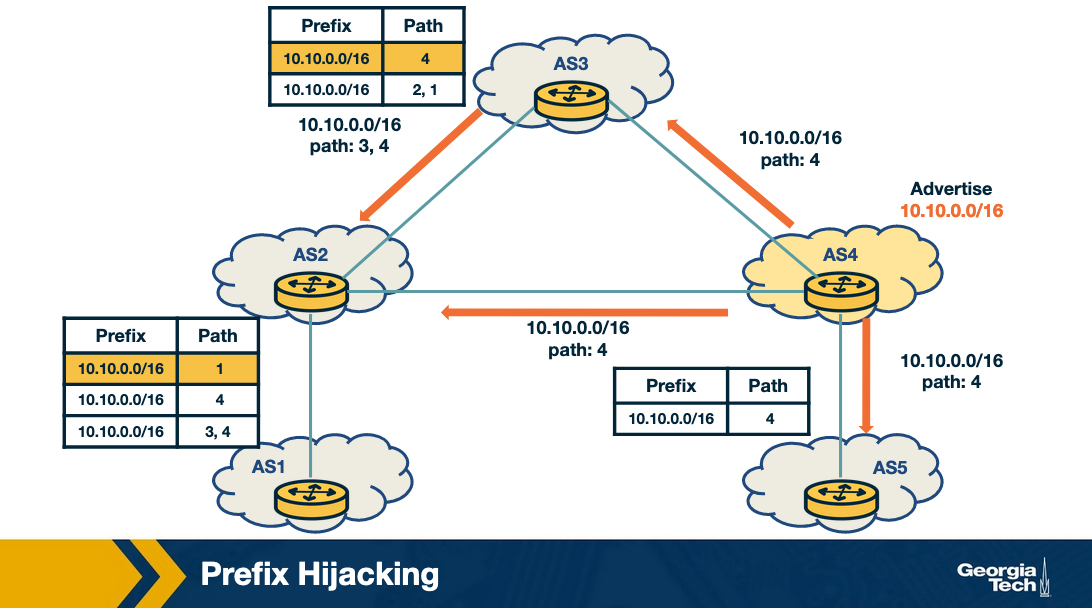
\includegraphics[width=.9\linewidth]{./MD_Figures/9_bgp_attacks_prefix_hijacking_1.png}
\caption{\label{fig:org49276b5}Prefix Hijacking}
\end{figure}

\subsection{Attack Scenario: Hijacking a path}
\label{sec:org5724c29}

In the figure below we see an attack scenario where a legitimate path is hijacked. 

In this scenario, the attacker manipulates received updates before propagating them to neighbors. 

\begin{enumerate}
\item AS1 advertises the prefix 10.10.0.0/16.
\item AS2 and AS3 receive and propagate legitimately the path for the prefix.
\item At AS4, the attacker compromises the update for the path by changing it to 4,1 and propagates it to the neighbors AS3, AS2, and AS5. Therefore it claims that it has direct link to AS1 so that others believe the new false path.
\item AS5 receives the false path (4,1)  “believes” the new false path and it adopts it. But the rest of the ASes don’t adopt the new path because they either have an shorter path already or an equally long path to AS1 for the same prefix.
\end{enumerate}

The key observation here is that the attacker does not need not to announce a new prefix, but rather it manipulates an advertisement before propagating it.

\begin{figure}[htbp]
\centering
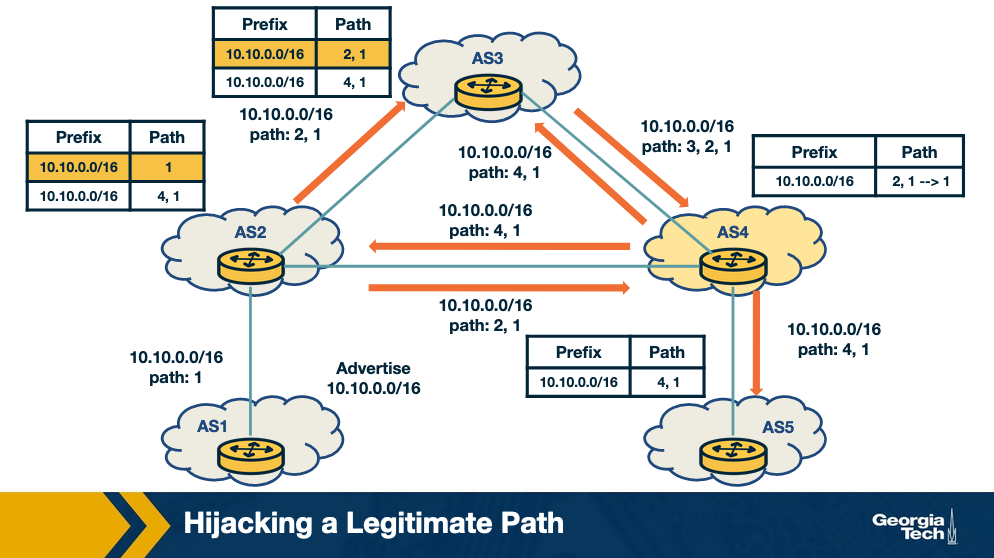
\includegraphics[width=.9\linewidth]{./MD_Figures/9_bgp_attacks_hijacking_path_1.png}
\caption{\label{fig:org21b1afd}Hijacking a Legitimate Path}
\end{figure}

\section{Defending against BGP Hijacking: An example detection system}
\label{sec:org18cd761}

In this section we will look at some high level ideas behind detecting BGP hijacking. ARTEMIS is a system that is run locally by network operators to safeguard its own prefixes against malicious BGP hijacking attempts. The authors of the ARTEMIS paper (Sermpezis et al) describe a self-operated manner of prefix hijacking detection.

The key ideas behind ARTEMIS are:

\begin{enumerate}
\item \textbf{A configuration file}: where all the prefixes owned by the network are listed here for reference. This configuration file is populated by the network operator.
\item \textbf{A mechanism for receiving BGP updates}: this allows receiving updates from local routers and monitoring services. This is built into the system
\end{enumerate}

Using the local configuration file as a reference, for the received BGP updates, ARTEMIS can check for prefixes and AS-PATH fields and trigger alerts when there are anomalies.

\begin{figure}[htbp]
\centering
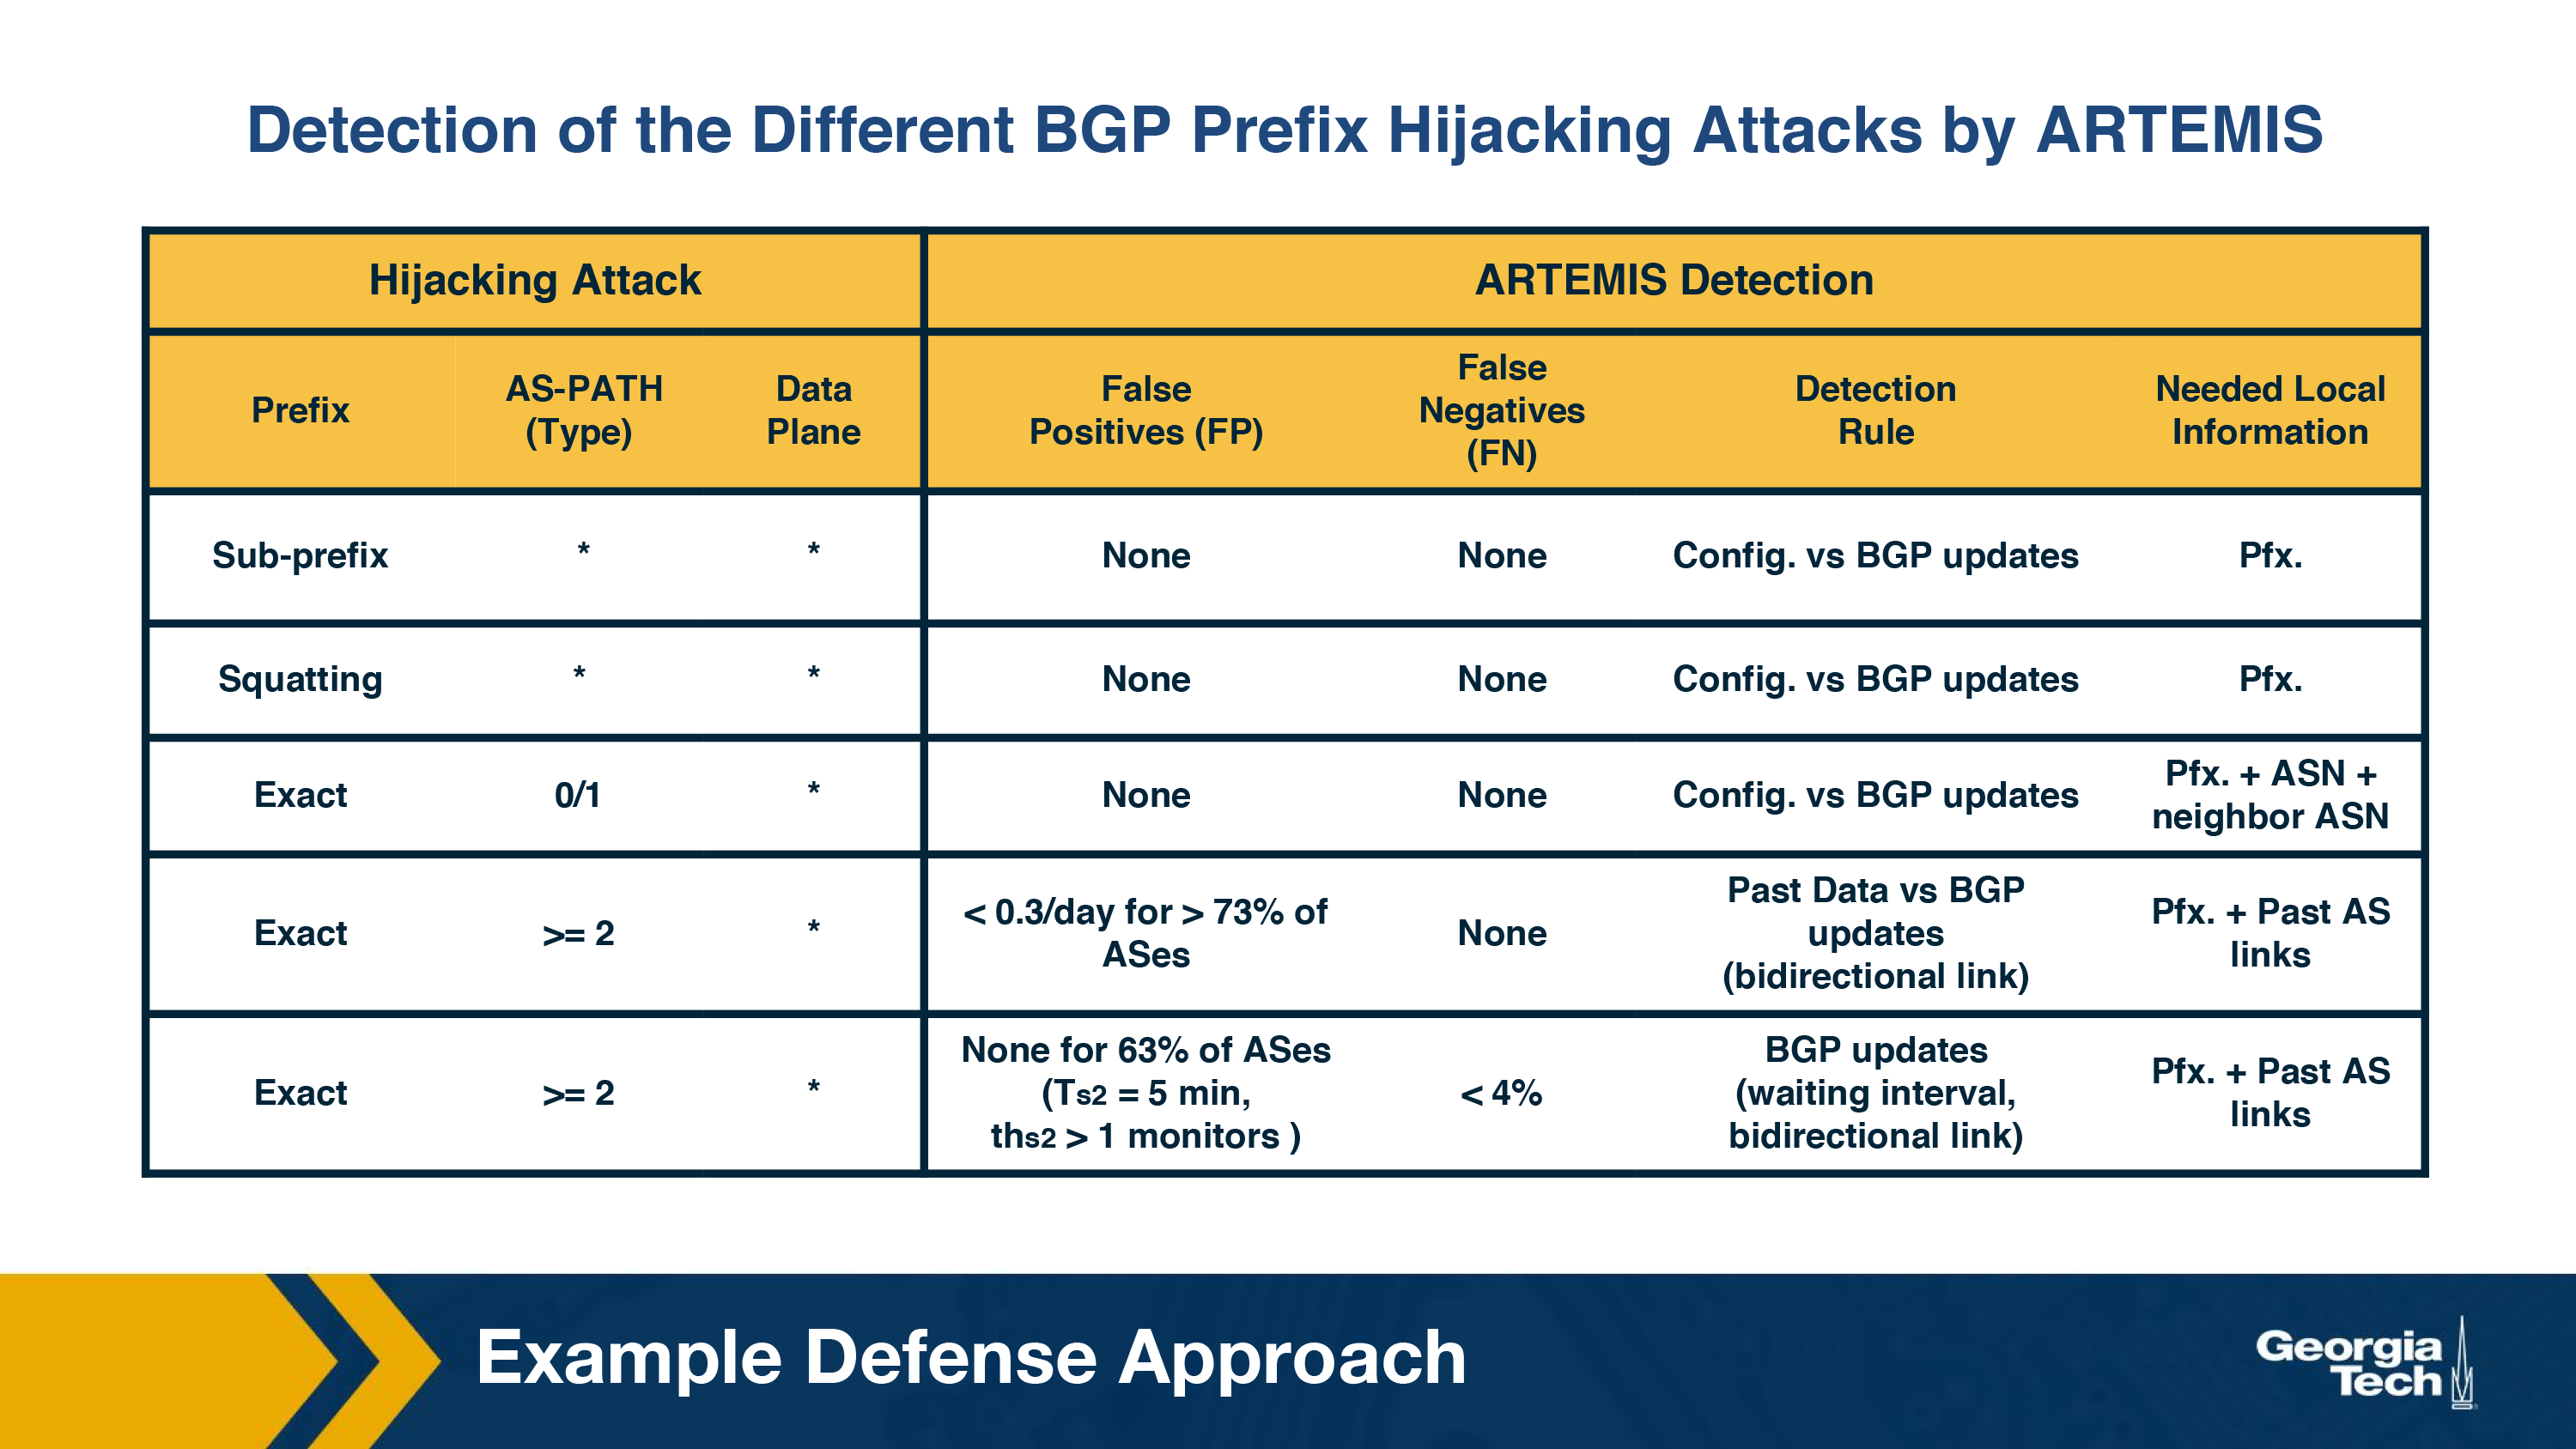
\includegraphics[width=.9\linewidth]{./MD_Figures/9_defending_bgp_attack_1.png}
\caption{\label{fig:org572da35}Example Defense Approach}
\end{figure}

A point of consideration in BGP hijacking detection is the performance of False Positive (FP) and False Negative (FN) rates when we use different detection criteria. We ideally want a system with the least number of FPs and FNs that are inconsequential. The ARTEMIS system also allows the network operator to choose between a) accuracy and speed, and b) FN which are inconsequential (less impact on control plane) for less FP.


\section{Defending against BGP Hijacking: Example Mitigation Techniques}
\label{sec:orgd8c56bd}

For a system that protects against BGP hijacking attacks with less manual intervention, we need automated ways of mitigation from BGP hijacking attacks. The ARTEMIS system uses two automated techniques in mitigating these attacks:

\begin{enumerate}
\item \textbf{Prefix deaggregation}: In a BGP attack scenario, the affected network can either contact other networks or it can simply deaggregate the prefixes that were targeted by announcing more specific prefixes of a certain prefix. Remember our prior discussion of YouTube’s services being attacked by Pakistan Telecom. The targeted prefix was 208.65.153.0/24. Within 90 minutes, YouTube started announcing 208.65.153.128/25 and 208.65.153.0/25, thereby counteracting the attack. Although the event required a long term solution, an immediate mitigation was required for services to come back online.

\item \textbf{Mitigation with Multiple Origin AS (MOAS)}: Here, the idea is to have third party organizations and service providers do BGP announcements for a given network. It is akin to the current model that exists for legitimizing network traffic by third parties that mitigate DDoS attacks. When a BGP hijacking event occurs, the following steps occur:
\end{enumerate}

a. The third party receives a notification and immediately announces from their locations the hijacked prefix(es). 

b. In this way, network traffic from across the world is attracted to the third party organization, which then scrubbs it and tunnels it to the legitimate AS

The authors of the ARTEMIS paper put forth two main findings from their research  work:

\begin{enumerate}
\item \textbf{Outsource the task of BGP announcement to third parties}: To combat against BGP hijacking attacks, having even just one single external organization to mitigate BGP attacks is highly effective against BGP attacks.
\item \textbf{Comparison of outsourcing BGP announcements vs prefix filtering}: When compared against prefix filtering, which is the current standard defense mechanism, the research work found that filtering is less optimal when compared against BGP announcem
\end{enumerate}


\section{DDoS: Background and Spoofing}
\label{sec:org9a01f01}

In this topic, we are talking about another type of abuse; the Denial of Service Attack (DDoS). We are also talking about how attackers amplify DDoS attacks by using an additional technique called Spoofing. 

A Distributed Denial of Service (DDoS) attack is an attempt to compromise a server or network resources with a flood of traffic. To achieve this, the attacker first compromises and deploys flooding servers (slaves). 

Later, when initiating an attack, the attacker instructs these flooding servers to send a high volume of traffic to the victim. This results in the victim host either becoming unreachable or in exhaustion of its bandwidth.

\begin{figure}[htbp]
\centering
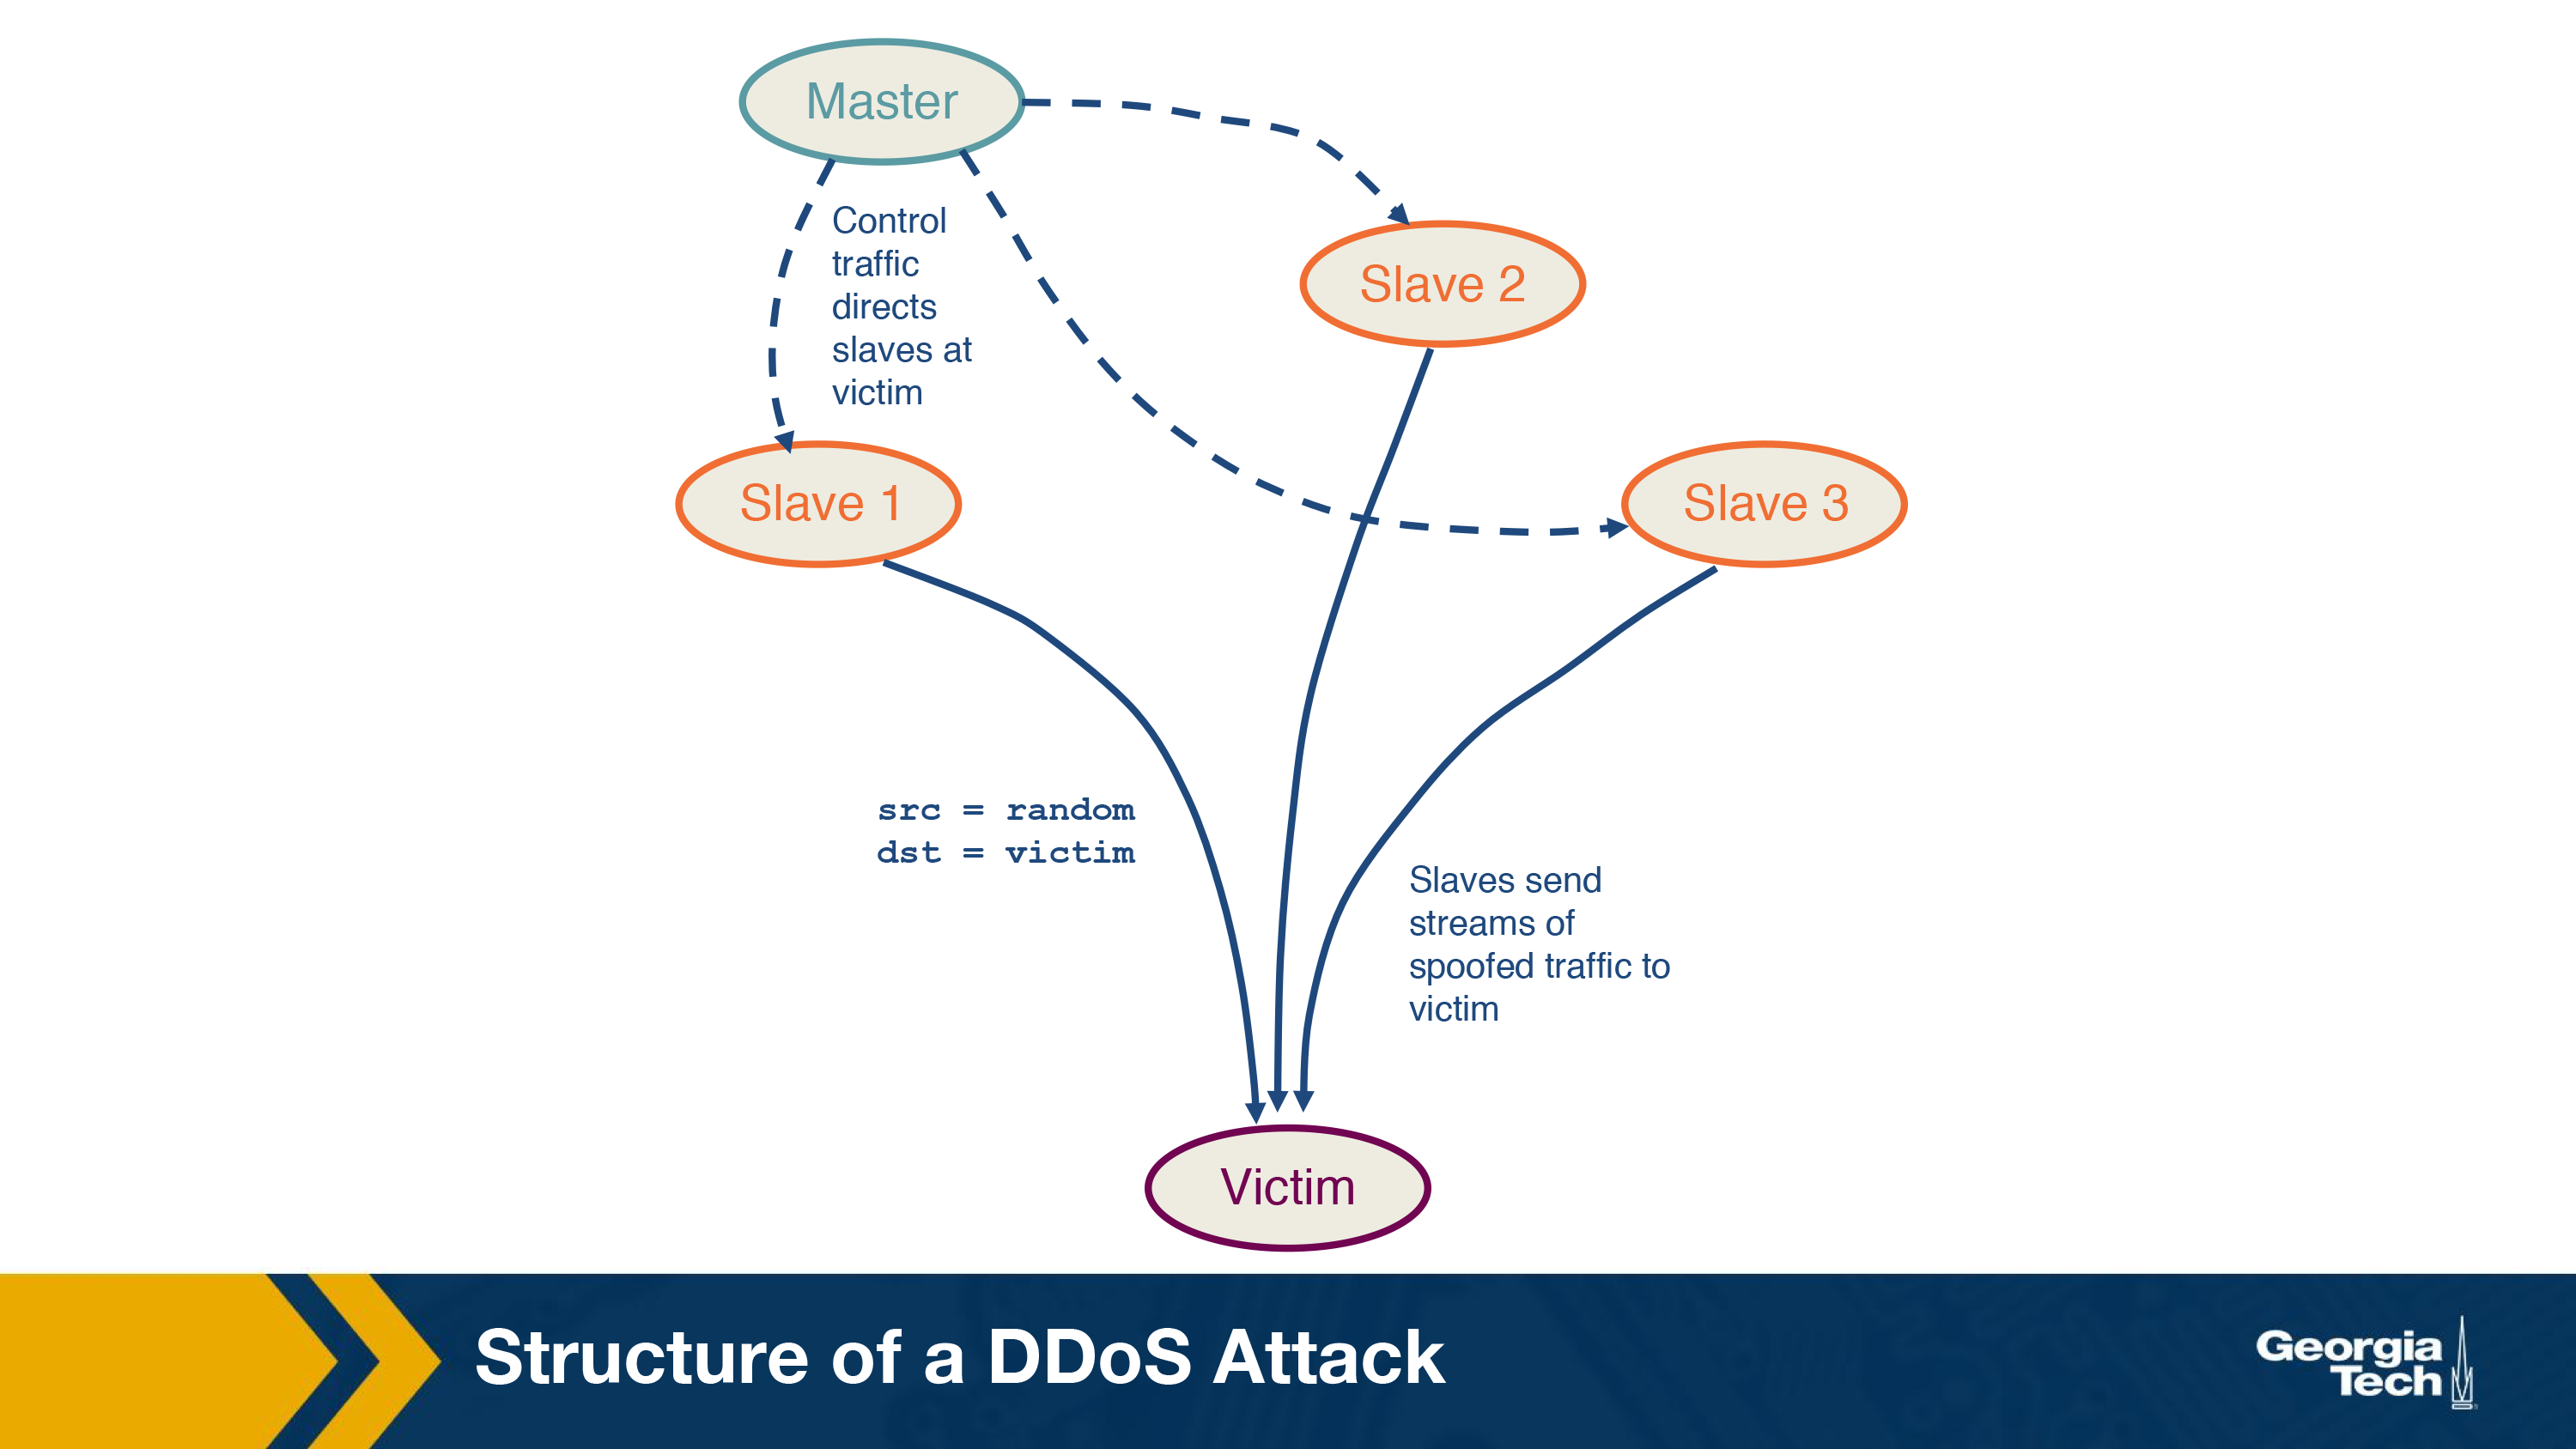
\includegraphics[width=.9\linewidth]{./MD_Figures/9_structure_of_ddos.png}
\caption{\label{fig:org9ac69fd}Structure of DDoS Attack}
\end{figure}

In the above figure, the master host, controlled by the attacker, sends control messages to the three compromised slaves directing them to send a huge amount of traffic to the victim. The packets sent from the slave contain the source address as a random IP address and the destination as the victim’s IP address. This master slave configuration amplifies the intensity of the attack while also making it difficult to protect against it. The attack traffic sent by the slaves contain spoofed source addresses making it difficult for the victim to track the slaves. Also, since the traffic is sent from multiple sources, it’s harder for the victim to isolate and block the attack traffic.

\subsection{Spoofing}
\label{sec:orgad75eb0}

IP spoofing is the act of setting a false IP address in the source field of a packet with the purpose of impersonating a legitimate server. In DDoS attacks, this can happen in two forms. In the first form, the source IP address is spoofed, resulting in the response of the server sent to some other client instead of the attacker’s machine. This results in wastage of network resources and the client resources while also causing denial of service to legitimate users. 

In the second type of attack, the attacker sets the same IP address in both the source and destination IP fields. This results in the server sending the replies to itself, causing it to crash.

\section{DDoS: Reflection and Amplification}
\label{sec:orgaba95c5}

In this topic we are continuing our discussion on DDoS and we explore two more techniques that the attackers are using to amplify the impact of the attack; namely the techniques of reflection and amplification.



\subsection{Reflection and amplification attacks.}
\label{sec:orgd785d03}

In a reflection attack, the attackers use a set of reflectors to initiate an attack on the victim. A reflector is any server that sends a response to a request. For example, any web server or a DNS server would return a SYN ACK in response to a SYN packet as part of TCP handshake. Other examples include query responses sent by a server or Host Unreachable responses to a particular IP. 

Here, the master directs the slaves to send spoofed requests to a very large number of reflectors, usually in the range of 1 million. The slaves set the source address of the packets to the victim’s IP address, thereby redirecting the response of the reflectors to the victim. Thus, the victim receives responses from millions of reflectors resulting in exhaustion of its bandwidth. In addition, the resources of the victim is wasted in processing these responses, making it unable to respond to legitimate requests. This forms the basis of a reflection attack. Let’s consider the below figure.


\begin{figure}[htbp]
\centering
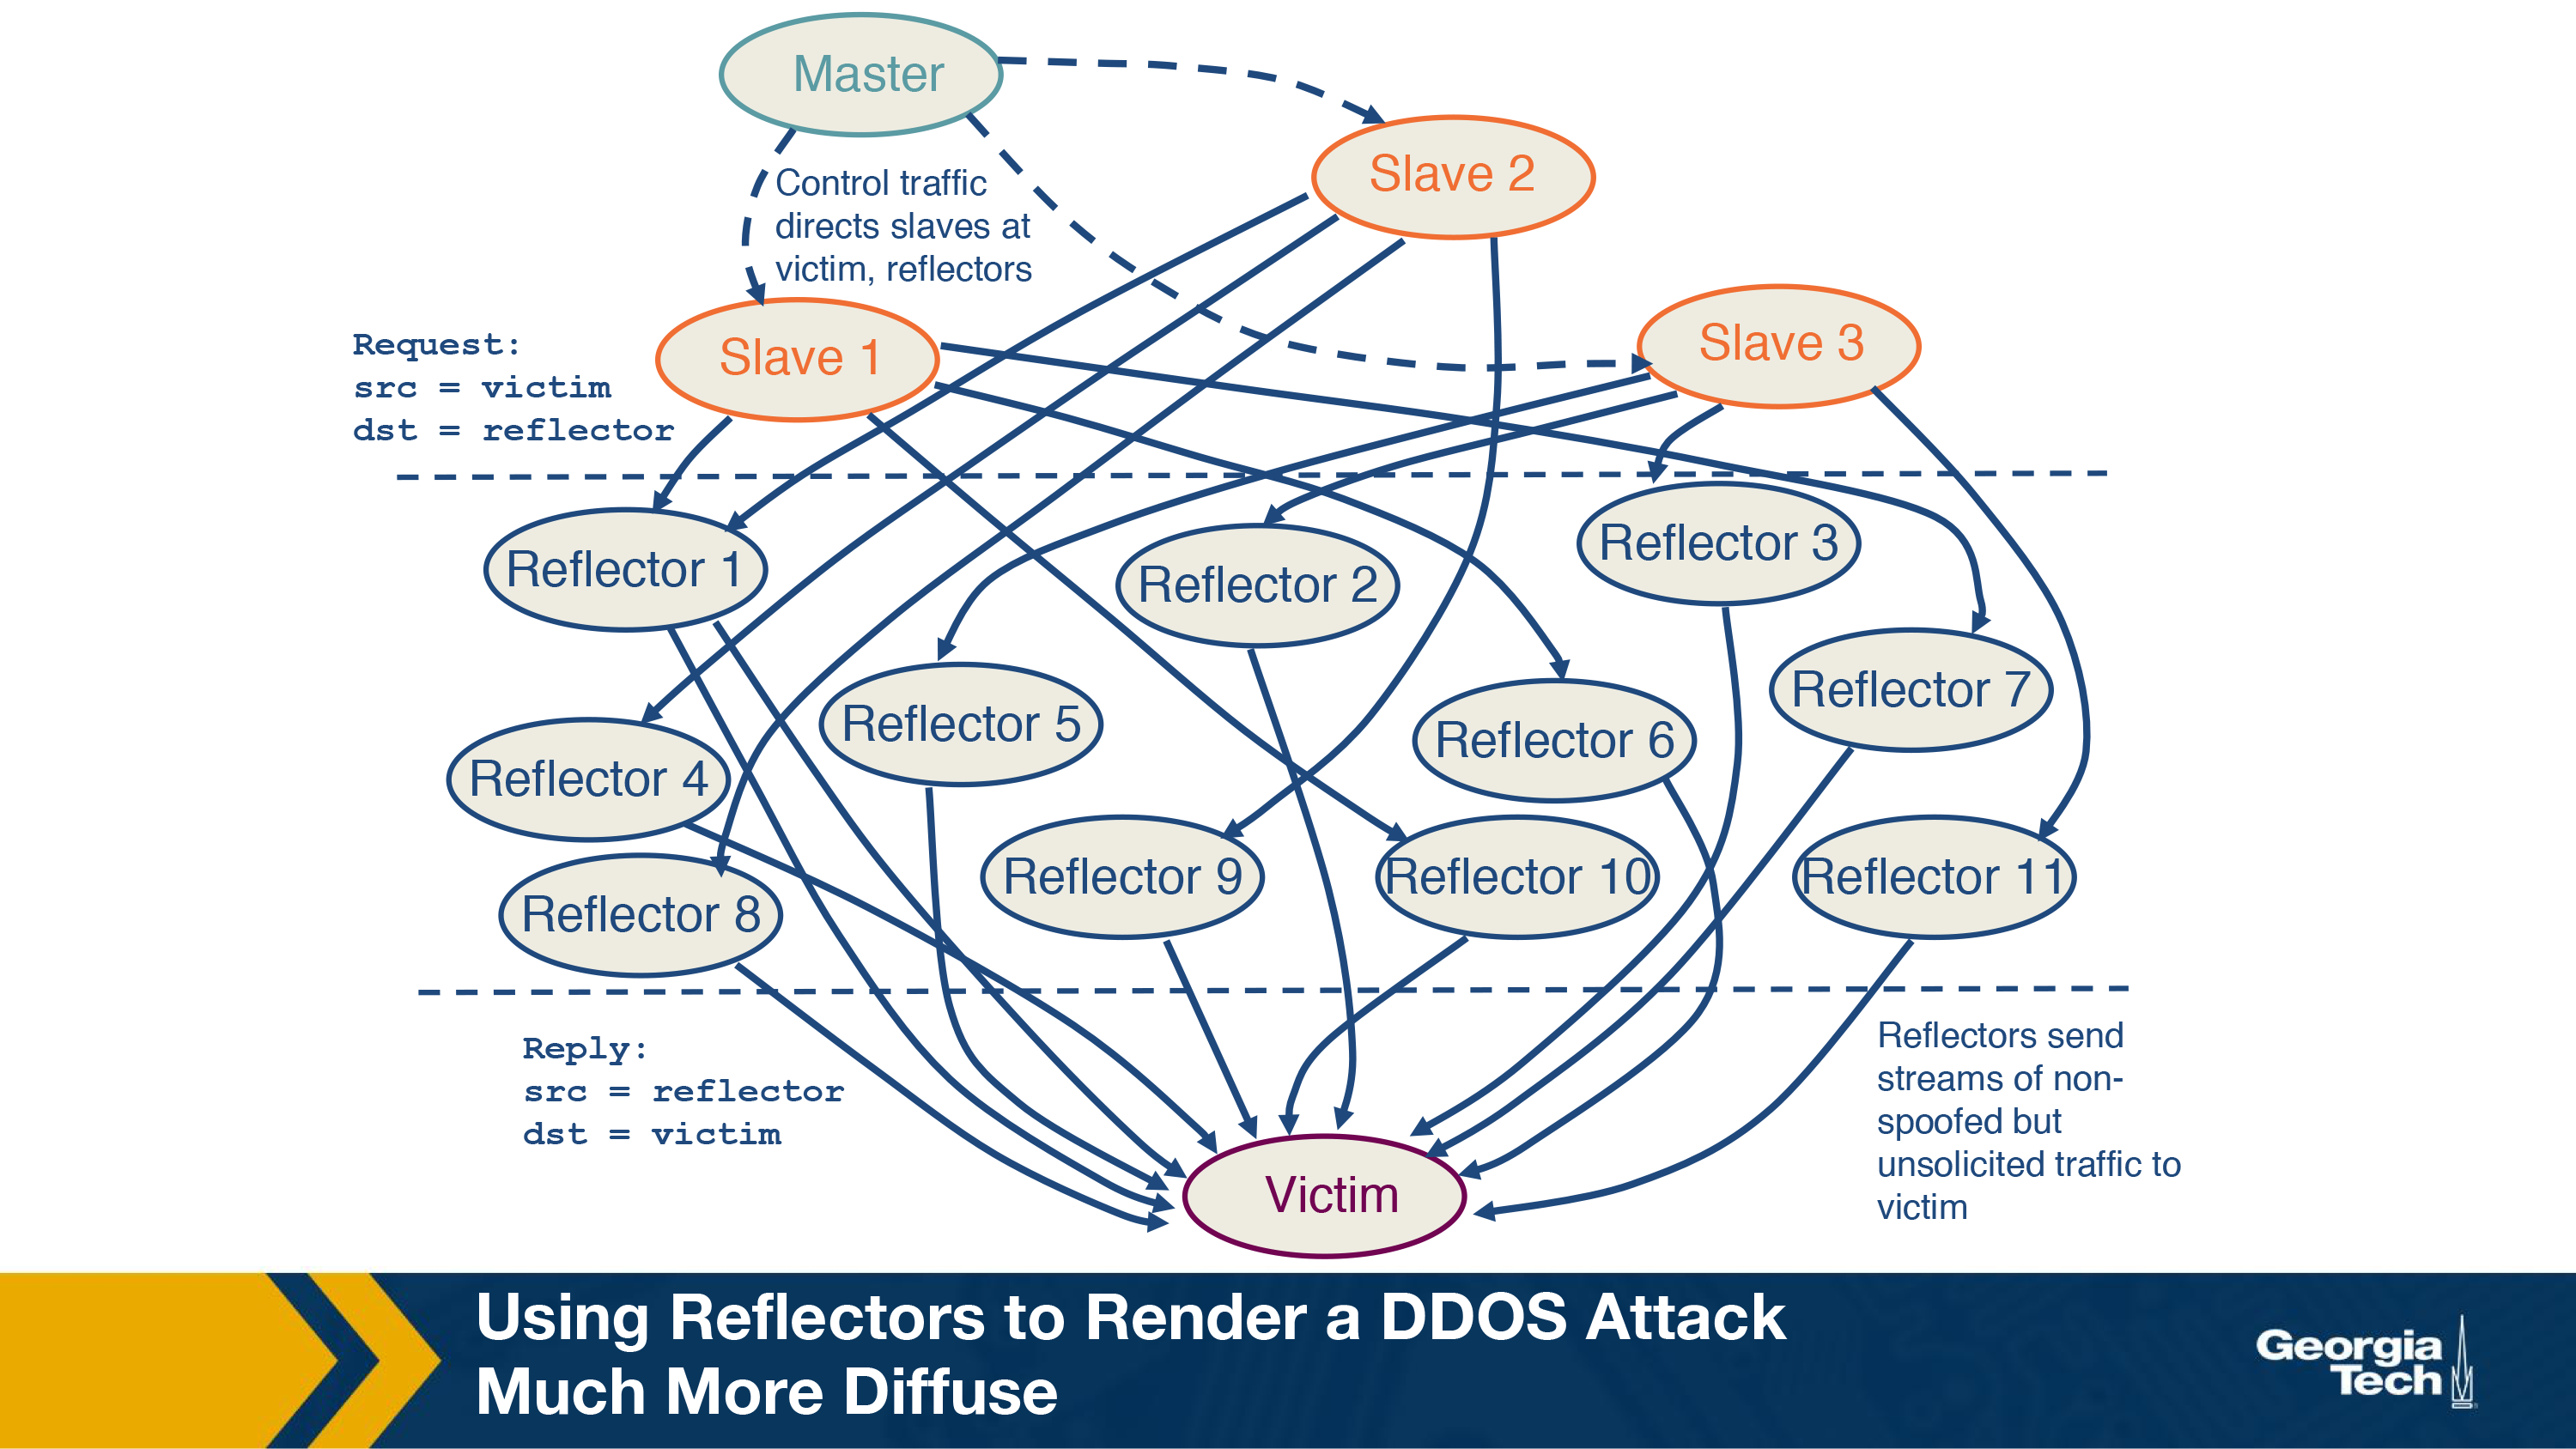
\includegraphics[width=.9\linewidth]{./MD_Figures/9_reflection_amplification_ddos.png}
\caption{\label{fig:orgea55325}Using Reflectors to Render a DDoS Attack Much More Diffuse}
\end{figure}


The master commands the three slaves to send spoofed requests to the reflectors, which in turn sends traffic to the victim. This is in contrast with the conventional DDoS attack we saw in the previous section, where the slaves directly send traffic to the victim. Note that the victim can easily identify the reflectors from the response packets. However, the reflector cannot identify the slave sending the spoofed requests. 

If the requests are chosen in such a way that the reflectors send large responses to the victim, it is a reflection and amplification attack. Not only would the victim receive traffic from millions of servers, the response sent would be large in size, making it further difficult for the victim to handle it.

\section{Defenses Against DDoS Attacks}
\label{sec:org2972f8d}

In this topic we are providing an overview of the tools that we have to help with a DDoS attack is under the way or to help deter the attack.

\subsection{Traffic Scrubbing Services}
\label{sec:orgde1efa5}

A scrubbing service diverts the incoming traffic to a specialized server, where the traffic is “scrubbed” into either clean or unwanted traffic. The clean traffic is then sent to its original destination. Although this method offers fine-grained filtering of the packets, there are monetary costs required for an in-time subscription, setup and other recurring costs. The other limitations include reduced effectiveness due to per packet processing and challenges in handling Tbps level attacks. There’s also a possibility of decreased performance as the traffic may be rerouted and becoming susceptible to evasion attacks.



\subsection{ACL Filters}
\label{sec:org7434d75}

Access Control List filters are deployed by ISPs or IXPs at their AS border routers to filter out unwanted traffic. These filters, whose implementation depends on the vendor-specific hardware, are effective when the hardware is homogeneous and the deployment of the filters can be automated. The drawbacks of these filters include limited scalability and since the filtering does not occur at the ingress points, it can exhaust the bandwidth to a neighboring AS.



\subsection{BGP Flowspec}
\label{sec:orged75e39}

The flow specification feature of BGP, called Flowspec, helps to mitigate DDoS attacks by supporting the deployment and propagation of fine-grained filters across AS domain borders. It can be designed to match a specific flow or be based on packet attributes like length and fragment. It can also be based on the drop rate limit. Although flowspec has been effective in intra-domain environment, it is not so popular in inter-domain environments as it depends on trust and cooperation among competitive networks. 

BGP Flowspec is an extension to the BGP protocol which allows rules to be created on the traffic flows and take corresponding actions. This feature of BGP can help mitigate DDoS attacks by specifying appropriate rules. The AS domain borders supporting BGP Flowspec are capable of matching packets in a specific flow based on a variety of parameters such as source IP, destination IP, packet length, protocol used, etc.

The following table shows the available components with an example for FlowSpec:

\begin{figure}[htbp]
\centering
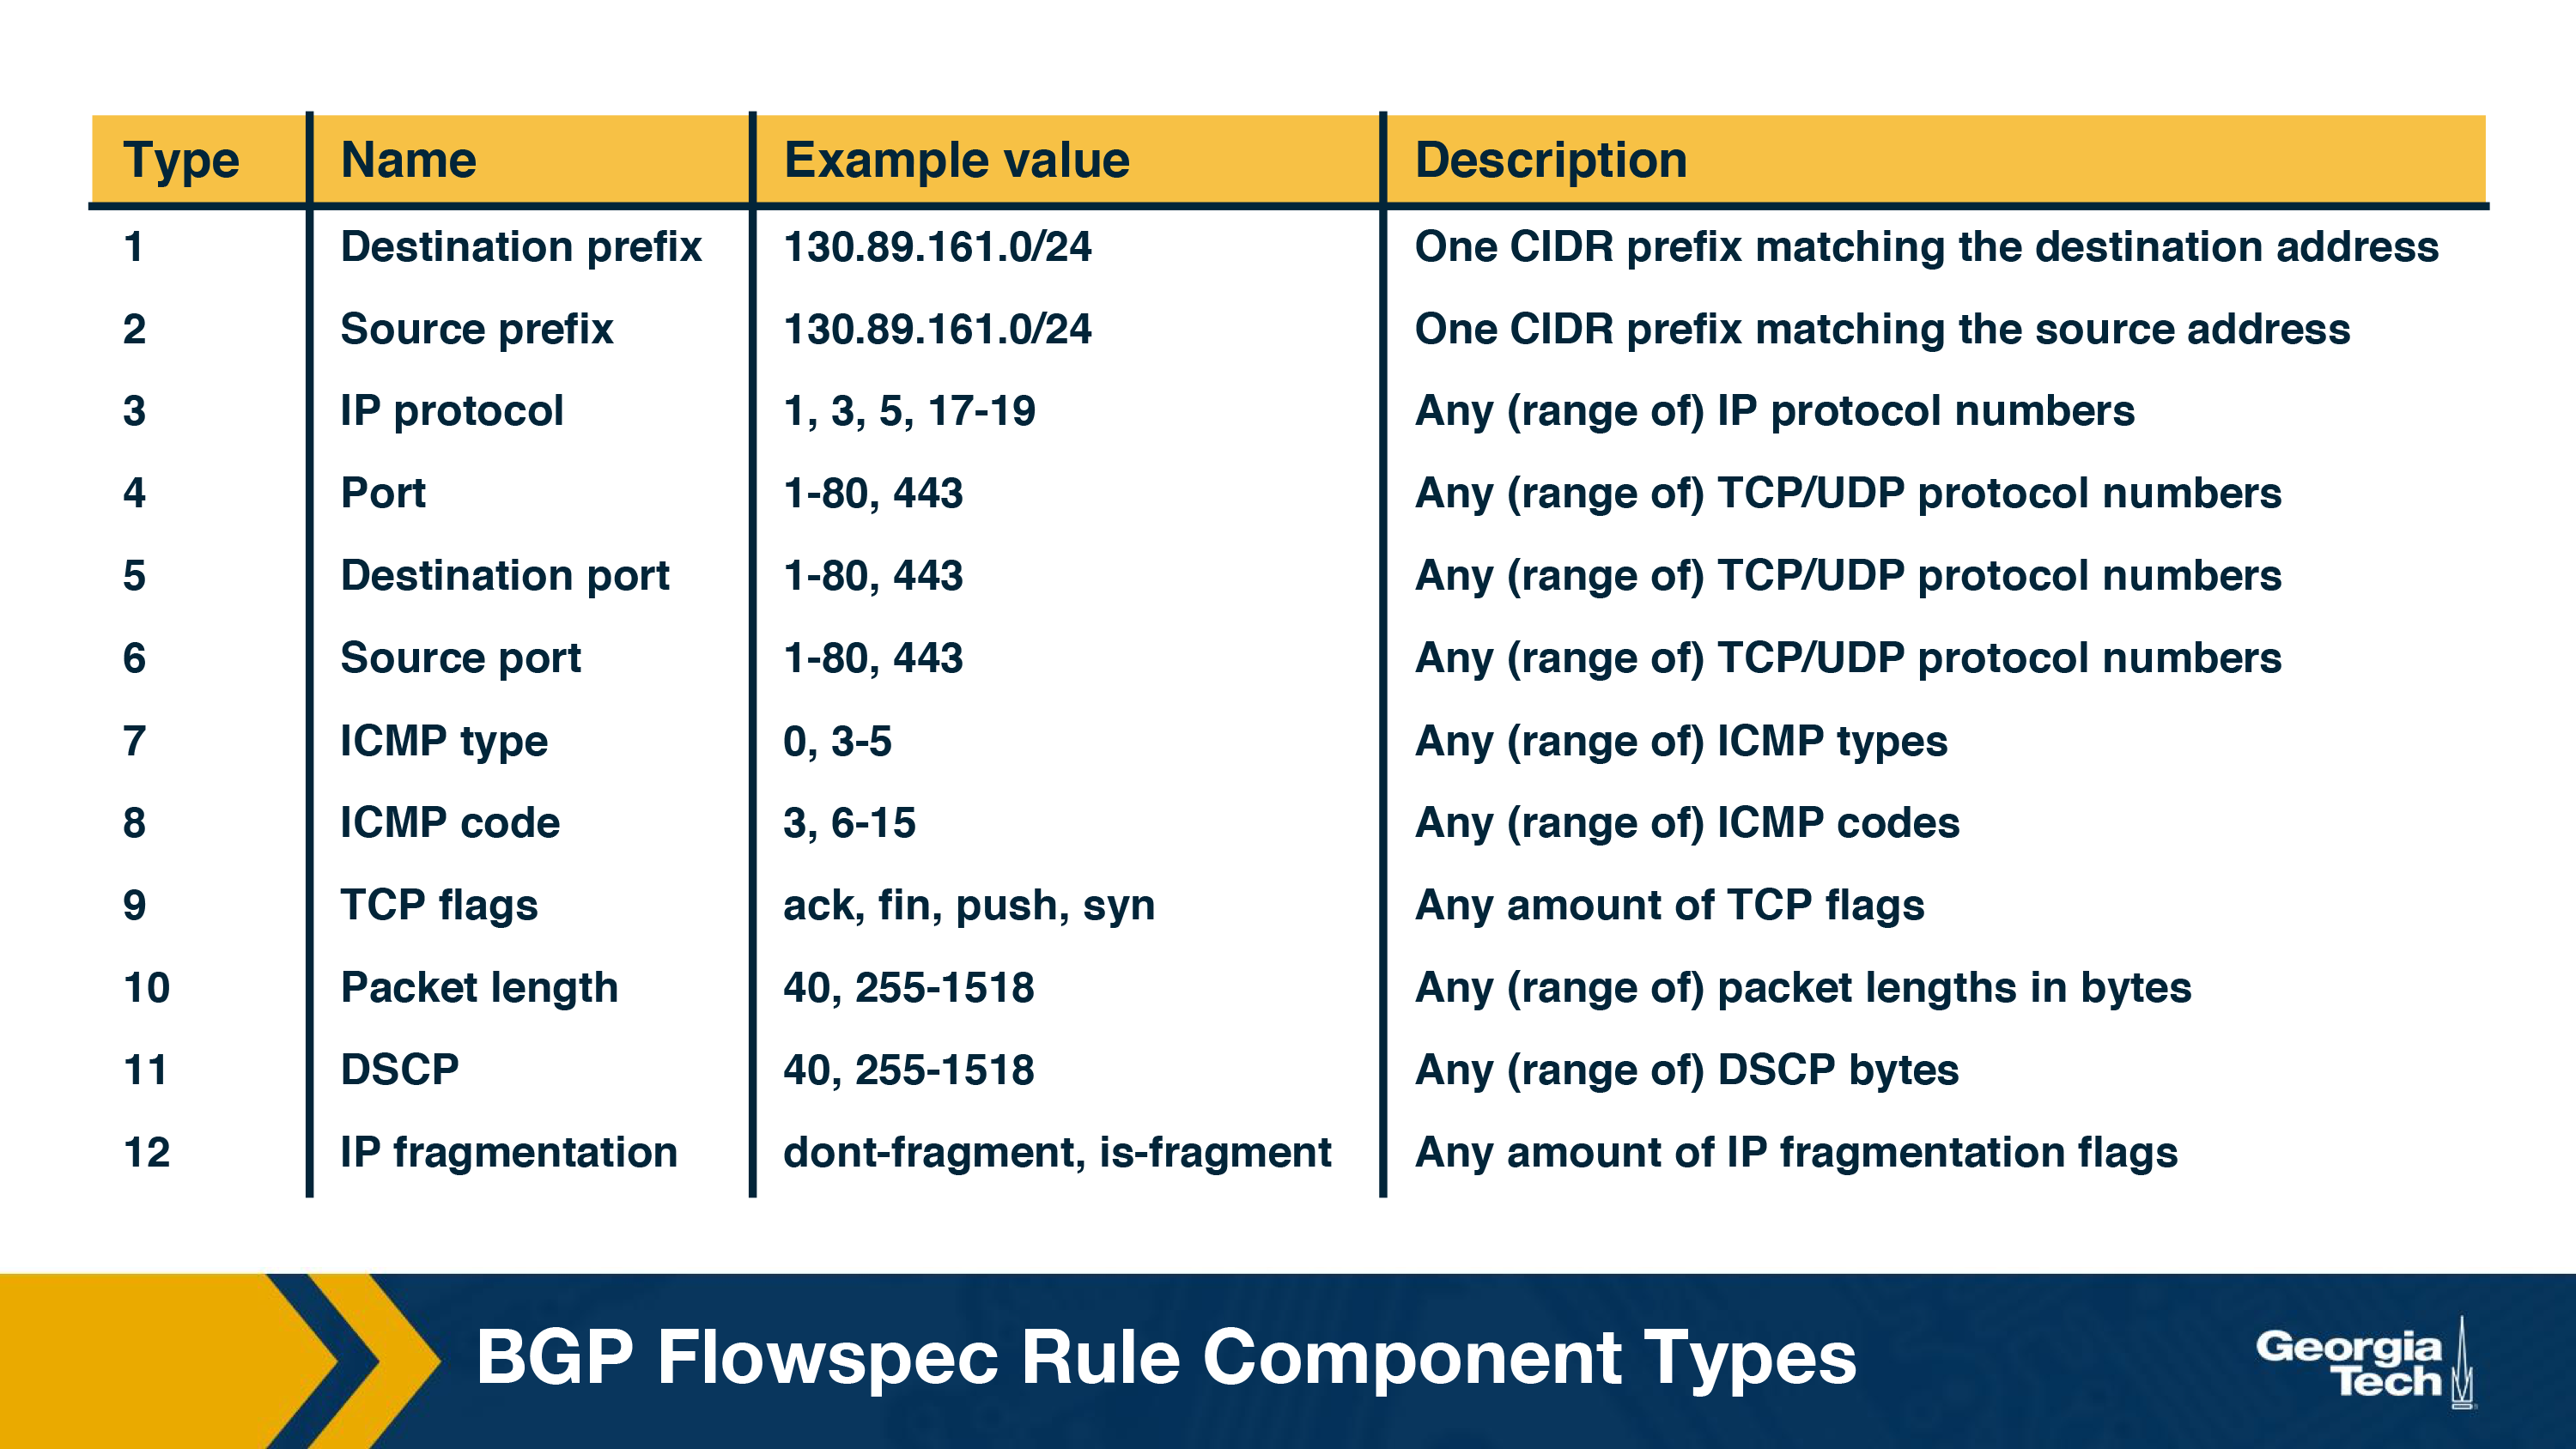
\includegraphics[width=.9\linewidth]{./MD_Figures/9_bgp_flowspec.png}
\caption{\label{fig:org12f699e}BGP FlowSpec}
\end{figure}


\textbf{BGP Flowspec example}: The following flow specification rule (specified here in a dictionary format) filters all HTTP/HTTPS traffic from port 80 and 443 to one of the Google servers with IP 172.217.19.195 from subnet 130.89.161.0/24.

\begin{verbatim}
{ 

   "type 1": "172.217.19.195/32”

   “type 2": "130.89.161.0/24" 

   "type 3": [6], 

   "type 5": [80, 443], 

   "action": { 

	    "type ": "traffic-rate", 

	    “value ": "0" 
   }
} 
\end{verbatim}

A “traffic-rate” action with value 0 discards the traffic. The other possible actions include rate limiting, redirecting or filtering. If no rule is specified, the default action for a rule is to accept the incoming traffic. 


In contrast to ACL filters, FlowSpec leverages the BGP control plane making it easier to add rules to all the routers simultaneously. Although FlowSpec is seen to be effective in intra-domain environment, it is not so popular in inter-domain environments as it depends on trust and cooperation among competitive networks. Also, it might not scale for large attacks where the attack traffic originates from multiple sources as it would multiple rules or combining the sources into one prefix. 

\section{DDoS Mitigation Techniques: BGP Blackholing}
\label{sec:org166a85b}

In this topic, we will talk about a technique called BGP blackholing, that is a countermeasure to mitigate a DDoS attack. 

With this mechanism, all the attack traffic to a targeted DoS destination is dropped to a null location. The premise of this approach is that the traffic is stopped closer to the source of the attack and before it reaches the targeted victim. For a high volume attack, it proves to be an effective strategy when compared to other mitigation options. 

This technique is implemented either with the help of the upstream provider or with the help of the IXP (if the network is peering at an IXP). With this technique, the victim AS uses BGP to communicate the attacked destination prefix to its upstream AS, which then drops the attack traffic towards this prefix. Then either the provider (or the IXP) will advertise a more specific prefix and modifying the next-hop address that will divert the attack traffic to a null interface. The blackhole messages are tagged with a specific BGP blackhole community attribute, usually publicly available, to differentiate it from the regular routing updates. 

Let's look at the scenario, where blackholing is implemented with the help of an upstream provider.

A network that offers blackholing service is known as a blackholing provider. It is also responsible for providing the blackholing community that should be used. Network or customer providers act as blackholing providers at the network edge. Internet Service Providers (ISPs) or Internet Exchange Points (IXPs) act as blackholing providers at the Internet core. 

If the blackholing provider is a peer or an upstream provider, the AS must announce its associated blackhole community along with the blackhole prefix. Let’s consider the below figure. Assume the IP 130.149.1.1 in AS2 is under attack.

\begin{figure}[htbp]
\centering
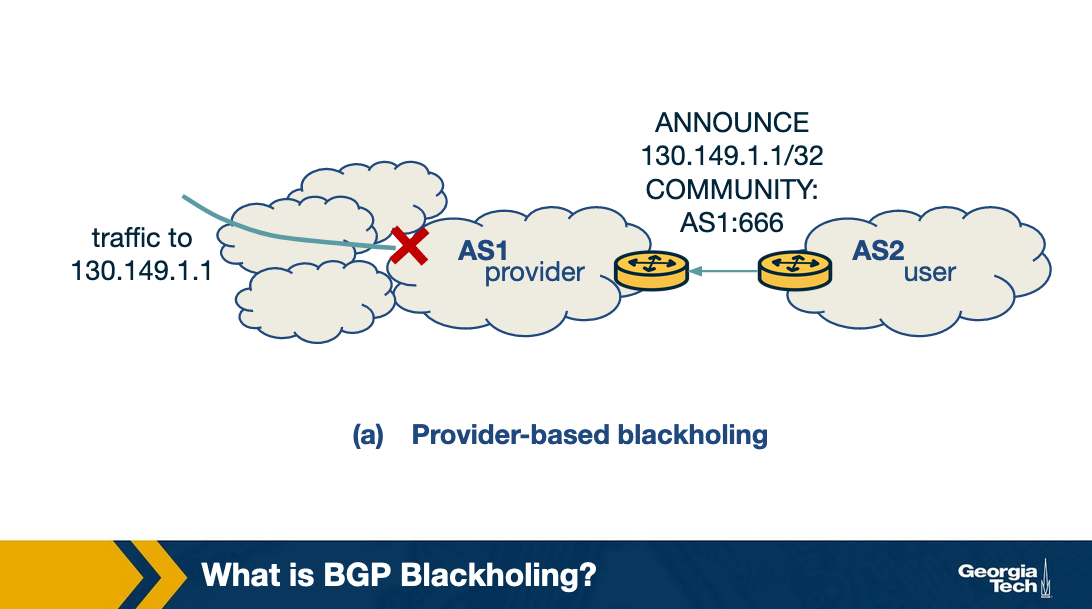
\includegraphics[width=.9\linewidth]{./MD_Figures/9_bgp_blackholing_1.png}
\caption{\label{fig:orge53aa62}Provider-based Blackholing}
\end{figure}

To mitigate this attack, AS2 (victim network) announces a blackholing message to AS1, which is the provider network. The message contains the IP 130.149.1.1/32, which is the host IP under attack and the community field set to AS1 : 666, which is the blackholing community of the AS1 provider. Once the provider receives the message, AS1 identifies it as a blackholing message since it contains its blackholing community and sets the next-hop field of the 130.149.1.1 IP to a blackholing IP, thereby effectively dropping all the incoming traffic to host 130.149.1.1. Thus, the victim host stops receiving the attack traffic that was sent to it. 

Let's look at the scenario, where blackholing is implemented with the help of the IXP where the victim network is already a participant.

In a similar manner, at IXPs, if the AS is a member of an IXP infrastructure and it is under attack, it sends the blackholing messages to the IXP route server when a member connects to the route server. The route server then announces the message to all the connected IXP member ASes, which then drops the traffic towards the blackholed prefix. The null interface to which the traffic should be sent is specified by the IXP. The blackholing message sent to the IXP should contain the IXP blackhole community as shown in the following figure. 

\begin{figure}[htbp]
\centering
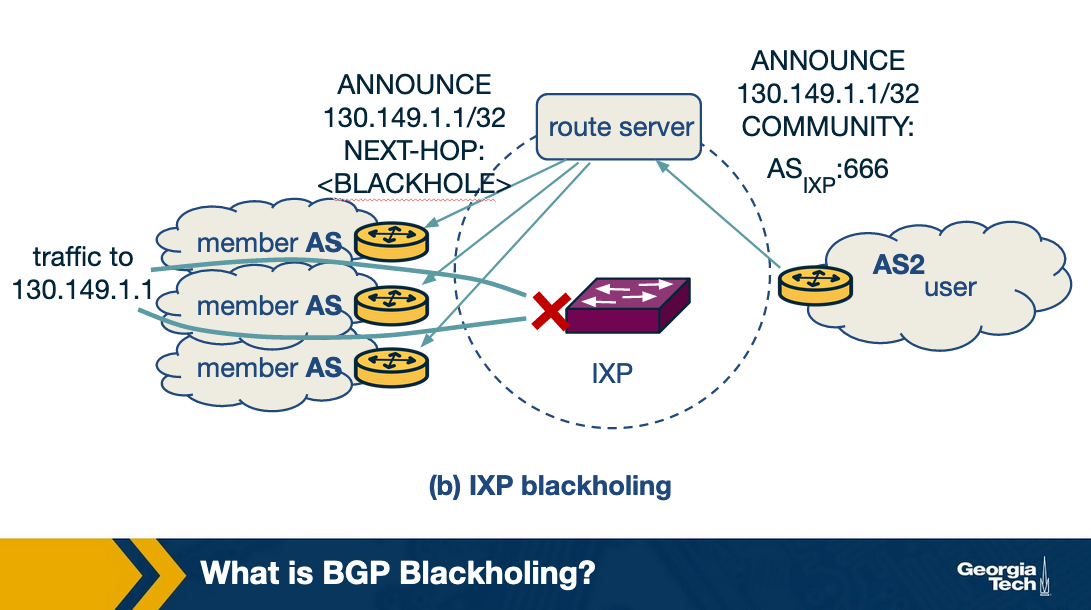
\includegraphics[width=.9\linewidth]{./MD_Figures/9_bgp_blackholing_2.png}
\caption{\label{fig:orgc3e5611}IXP Blackholing}
\end{figure}

Similar to the previous example, consider here an IP 130.149.1.1 in AS2 that is under attack. The victim AS, AS2 connects to the router server of the IXP and sends a BGP blackholing message. The message contains the IP under attack and the community field set to ASIXP : 666, which is the blackholing community of the IXP. The route server identifies it as a blackholing message and sets the next-hop of the 130.149.1.1 IP to a blackholing IP. It propagates this announcement to all its member ASes, which then drops all the traffic to host 130.149.1.1. 


\section{DDoS Mitigation Techniques: BGP Blackholing Limitations and Problems}
\label{sec:orgfce3913}

One of the major drawbacks of BGP blackholing is that the destination under attack becomes unreachable since all the traffic including the legitimate traffic is dropped. 

Consider the DDoS attack scenario in the given figure (a), where there is no mitigation strategy in place. In the control plane, the prefix 100.10.10.0/24 is advertised by AS1. Suppose a web service running on IP 100.10.10.10 comes under attack, which falls under AS1. As shown in the bottom section of figure (a), this results in unreachability of the service by users from both AS2 and AS3 as the network port in AS1 becomes overloaded. 

\begin{figure}[htbp]
\centering
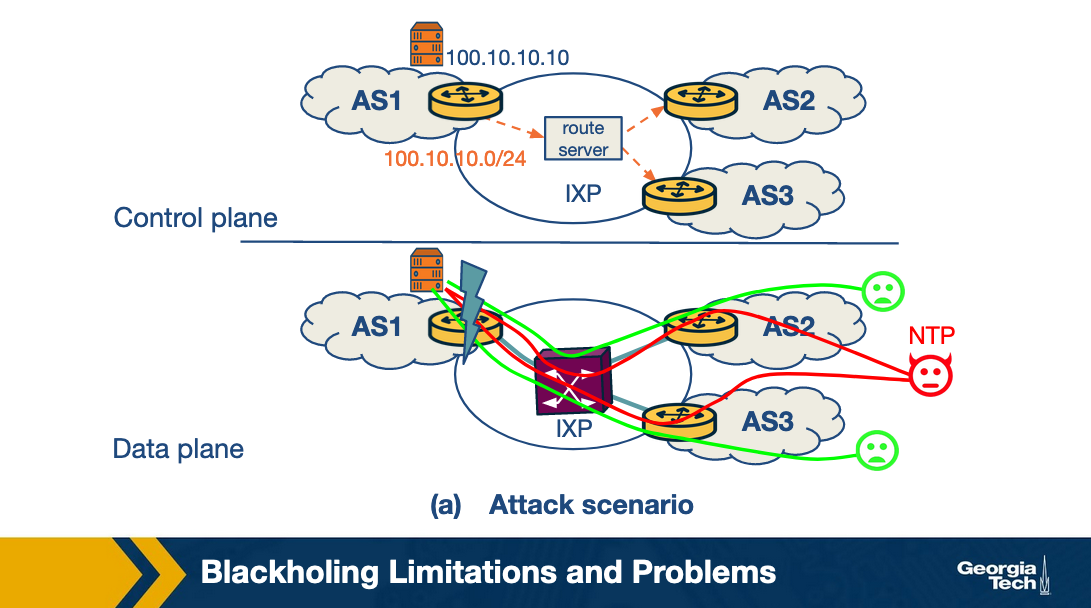
\includegraphics[width=.9\linewidth]{./MD_Figures/9_bgp_blackholing_attack_scenario.png}
\caption{\label{fig:org6edf63e}Attack Scenario}
\end{figure}

Now, consider the scenario where AS1 uses BGP blackholing to send an update to the IXP’s route server. The message contains the prefix 100.10.10.10/32 along with the IXP’s blackhole community (IXP\textsubscript{ASN}: 666). The route server propagates this update to the other ASes, AS2 and AS3, shown in the top section of figure (b). 

Let's assume the case where AS2 accepts the announcement and that AS3 rejects it. The possible reasons for an AS rejecting the announcement could include voluntarily choosing not to participate in blackholing, rejecting updates that require additional config changes or it could simply be that the AS made a misconfiguration mistake. 

Since AS2 accepts the announcement, the next hop IP for AS2 to reach the prefix under attack is changed to the IXP’s blackholing IP and traffic towards IP 100.10.10.10/32 via AS2 is dropped. However, this causes collateral damage since all the traffic including legitimate traffic via AS2 is dropped. 

\begin{figure}[htbp]
\centering
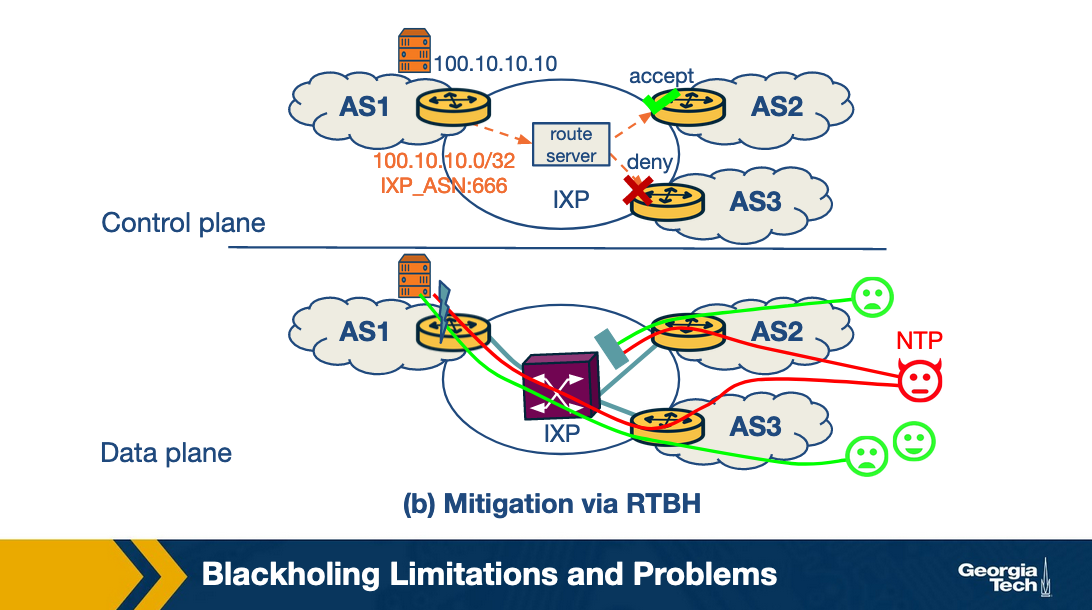
\includegraphics[width=.9\linewidth]{./MD_Figures/9_bgp_blackholing_mitigation.png}
\caption{\label{fig:org2d60aa7}Mitigation with RTBH}
\end{figure}

Also, since AS3 does not honor the announcement, it allows all the traffic including the legitimate and attacks traffic towards IP 100.10.10.10/32 to flow via AS3. 

As a result, and if the majority of the attack traffic is coming through AS3,  then the mitigation is ineffective. The same is true if a large number of peers do not accept the blackholing announcements. 

Let’s look at the traffic distribution during an attack at a large IXP, and gather some insights to understand the extent of the collateral damage caused by blackholing.

\begin{figure}[htbp]
\centering
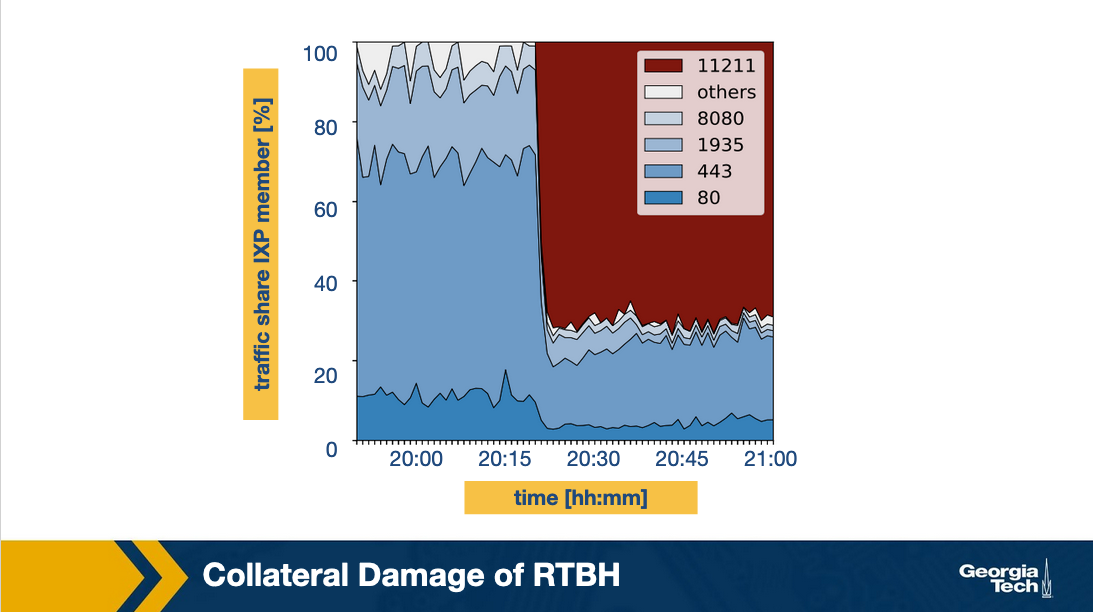
\includegraphics[width=.9\linewidth]{./MD_Figures/9_bgp_blackholing_collateral_damage.png}
\caption{\label{fig:org54899ed}Collateral Damage of RTBH}
\end{figure}

As can be seen from the above figure, the traffic mostly contains web traffic on ports 80 (HTTP) and 443 (HTTPS). The attack traffic, shown in red, is majorly from the UDP port 11211 and occupies almost 70\% of the entire traffic. This suggests an amplification attack. The ideal solution here would be to block the traffic only from the UDP port (11211), while allowing the remaining traffic from other ports to pass through. However, the blackholing service drops all traffic including the ones from other ports, which is still a significant amount. 
\end{document}
